\documentclass[11pt]{article}

    \usepackage[breakable]{tcolorbox}
    \usepackage{parskip} % Stop auto-indenting (to mimic markdown behaviour)
    

    % Basic figure setup, for now with no caption control since it's done
    % automatically by Pandoc (which extracts ![](path) syntax from Markdown).
    \usepackage{graphicx}
    % Maintain compatibility with old templates. Remove in nbconvert 6.0
    \let\Oldincludegraphics\includegraphics
    % Ensure that by default, figures have no caption (until we provide a
    % proper Figure object with a Caption API and a way to capture that
    % in the conversion process - todo).
    \usepackage{caption}
    \DeclareCaptionFormat{nocaption}{}
    \captionsetup{format=nocaption,aboveskip=0pt,belowskip=0pt}

    \usepackage{float}
    \floatplacement{figure}{H} % forces figures to be placed at the correct location
    \usepackage{xcolor} % Allow colors to be defined
    \usepackage{enumerate} % Needed for markdown enumerations to work
    \usepackage{geometry} % Used to adjust the document margins
    \usepackage{amsmath} % Equations
    \usepackage{amssymb} % Equations
    \usepackage{textcomp} % defines textquotesingle
    % Hack from http://tex.stackexchange.com/a/47451/13684:
    \AtBeginDocument{%
        \def\PYZsq{\textquotesingle}% Upright quotes in Pygmentized code
    }
    \usepackage{upquote} % Upright quotes for verbatim code
    \usepackage{eurosym} % defines \euro

    \usepackage{iftex}
    \ifPDFTeX
        \usepackage[T1]{fontenc}
        \IfFileExists{alphabeta.sty}{
              \usepackage{alphabeta}
          }{
              \usepackage[mathletters]{ucs}
              \usepackage[utf8x]{inputenc}
          }
    \else
        \usepackage{fontspec}
        \usepackage{unicode-math}
    \fi

    \usepackage{fancyvrb} % verbatim replacement that allows latex
    \usepackage{grffile} % extends the file name processing of package graphics
                         % to support a larger range
    \makeatletter % fix for old versions of grffile with XeLaTeX
    \@ifpackagelater{grffile}{2019/11/01}
    {
      % Do nothing on new versions
    }
    {
      \def\Gread@@xetex#1{%
        \IfFileExists{"\Gin@base".bb}%
        {\Gread@eps{\Gin@base.bb}}%
        {\Gread@@xetex@aux#1}%
      }
    }
    \makeatother
    \usepackage[Export]{adjustbox} % Used to constrain images to a maximum size
    \adjustboxset{max size={0.9\linewidth}{0.9\paperheight}}

    % The hyperref package gives us a pdf with properly built
    % internal navigation ('pdf bookmarks' for the table of contents,
    % internal cross-reference links, web links for URLs, etc.)
    \usepackage{hyperref}
    % The default LaTeX title has an obnoxious amount of whitespace. By default,
    % titling removes some of it. It also provides customization options.
    \usepackage{titling}
    \usepackage{longtable} % longtable support required by pandoc >1.10
    \usepackage{booktabs}  % table support for pandoc > 1.12.2
    \usepackage{array}     % table support for pandoc >= 2.11.3
    \usepackage{calc}      % table minipage width calculation for pandoc >= 2.11.1
    \usepackage[inline]{enumitem} % IRkernel/repr support (it uses the enumerate* environment)
    \usepackage[normalem]{ulem} % ulem is needed to support strikethroughs (\sout)
                                % normalem makes italics be italics, not underlines
    \usepackage{mathrsfs}
    

    
    % Colors for the hyperref package
    \definecolor{urlcolor}{rgb}{0,.145,.698}
    \definecolor{linkcolor}{rgb}{.71,0.21,0.01}
    \definecolor{citecolor}{rgb}{.12,.54,.11}

    % ANSI colors
    \definecolor{ansi-black}{HTML}{3E424D}
    \definecolor{ansi-black-intense}{HTML}{282C36}
    \definecolor{ansi-red}{HTML}{E75C58}
    \definecolor{ansi-red-intense}{HTML}{B22B31}
    \definecolor{ansi-green}{HTML}{00A250}
    \definecolor{ansi-green-intense}{HTML}{007427}
    \definecolor{ansi-yellow}{HTML}{DDB62B}
    \definecolor{ansi-yellow-intense}{HTML}{B27D12}
    \definecolor{ansi-blue}{HTML}{208FFB}
    \definecolor{ansi-blue-intense}{HTML}{0065CA}
    \definecolor{ansi-magenta}{HTML}{D160C4}
    \definecolor{ansi-magenta-intense}{HTML}{A03196}
    \definecolor{ansi-cyan}{HTML}{60C6C8}
    \definecolor{ansi-cyan-intense}{HTML}{258F8F}
    \definecolor{ansi-white}{HTML}{C5C1B4}
    \definecolor{ansi-white-intense}{HTML}{A1A6B2}
    \definecolor{ansi-default-inverse-fg}{HTML}{FFFFFF}
    \definecolor{ansi-default-inverse-bg}{HTML}{000000}

    % common color for the border for error outputs.
    \definecolor{outerrorbackground}{HTML}{FFDFDF}

    % commands and environments needed by pandoc snippets
    % extracted from the output of `pandoc -s`
    \providecommand{\tightlist}{%
      \setlength{\itemsep}{0pt}\setlength{\parskip}{0pt}}
    \DefineVerbatimEnvironment{Highlighting}{Verbatim}{commandchars=\\\{\}}
    % Add ',fontsize=\small' for more characters per line
    \newenvironment{Shaded}{}{}
    \newcommand{\KeywordTok}[1]{\textcolor[rgb]{0.00,0.44,0.13}{\textbf{{#1}}}}
    \newcommand{\DataTypeTok}[1]{\textcolor[rgb]{0.56,0.13,0.00}{{#1}}}
    \newcommand{\DecValTok}[1]{\textcolor[rgb]{0.25,0.63,0.44}{{#1}}}
    \newcommand{\BaseNTok}[1]{\textcolor[rgb]{0.25,0.63,0.44}{{#1}}}
    \newcommand{\FloatTok}[1]{\textcolor[rgb]{0.25,0.63,0.44}{{#1}}}
    \newcommand{\CharTok}[1]{\textcolor[rgb]{0.25,0.44,0.63}{{#1}}}
    \newcommand{\StringTok}[1]{\textcolor[rgb]{0.25,0.44,0.63}{{#1}}}
    \newcommand{\CommentTok}[1]{\textcolor[rgb]{0.38,0.63,0.69}{\textit{{#1}}}}
    \newcommand{\OtherTok}[1]{\textcolor[rgb]{0.00,0.44,0.13}{{#1}}}
    \newcommand{\AlertTok}[1]{\textcolor[rgb]{1.00,0.00,0.00}{\textbf{{#1}}}}
    \newcommand{\FunctionTok}[1]{\textcolor[rgb]{0.02,0.16,0.49}{{#1}}}
    \newcommand{\RegionMarkerTok}[1]{{#1}}
    \newcommand{\ErrorTok}[1]{\textcolor[rgb]{1.00,0.00,0.00}{\textbf{{#1}}}}
    \newcommand{\NormalTok}[1]{{#1}}

    % Additional commands for more recent versions of Pandoc
    \newcommand{\ConstantTok}[1]{\textcolor[rgb]{0.53,0.00,0.00}{{#1}}}
    \newcommand{\SpecialCharTok}[1]{\textcolor[rgb]{0.25,0.44,0.63}{{#1}}}
    \newcommand{\VerbatimStringTok}[1]{\textcolor[rgb]{0.25,0.44,0.63}{{#1}}}
    \newcommand{\SpecialStringTok}[1]{\textcolor[rgb]{0.73,0.40,0.53}{{#1}}}
    \newcommand{\ImportTok}[1]{{#1}}
    \newcommand{\DocumentationTok}[1]{\textcolor[rgb]{0.73,0.13,0.13}{\textit{{#1}}}}
    \newcommand{\AnnotationTok}[1]{\textcolor[rgb]{0.38,0.63,0.69}{\textbf{\textit{{#1}}}}}
    \newcommand{\CommentVarTok}[1]{\textcolor[rgb]{0.38,0.63,0.69}{\textbf{\textit{{#1}}}}}
    \newcommand{\VariableTok}[1]{\textcolor[rgb]{0.10,0.09,0.49}{{#1}}}
    \newcommand{\ControlFlowTok}[1]{\textcolor[rgb]{0.00,0.44,0.13}{\textbf{{#1}}}}
    \newcommand{\OperatorTok}[1]{\textcolor[rgb]{0.40,0.40,0.40}{{#1}}}
    \newcommand{\BuiltInTok}[1]{{#1}}
    \newcommand{\ExtensionTok}[1]{{#1}}
    \newcommand{\PreprocessorTok}[1]{\textcolor[rgb]{0.74,0.48,0.00}{{#1}}}
    \newcommand{\AttributeTok}[1]{\textcolor[rgb]{0.49,0.56,0.16}{{#1}}}
    \newcommand{\InformationTok}[1]{\textcolor[rgb]{0.38,0.63,0.69}{\textbf{\textit{{#1}}}}}
    \newcommand{\WarningTok}[1]{\textcolor[rgb]{0.38,0.63,0.69}{\textbf{\textit{{#1}}}}}


    % Define a nice break command that doesn't care if a line doesn't already
    % exist.
    \def\br{\hspace*{\fill} \\* }
    % Math Jax compatibility definitions
    \def\gt{>}
    \def\lt{<}
    \let\Oldtex\TeX
    \let\Oldlatex\LaTeX
    \renewcommand{\TeX}{\textrm{\Oldtex}}
    \renewcommand{\LaTeX}{\textrm{\Oldlatex}}
    % Document parameters
    % Document title
    \title{\textbf{Pattern Recognition}\\\textbf{Assignment 1}}
\author{\textbf{Ziad Reda Saad - 19015717}\\
\textbf{Ali Mones Abd El-Mohsen - 2001094}\\
\textbf{Marwan Mostafa Abd El-Kader - 20011867}}
    
    
    
    
    
% Pygments definitions
\makeatletter
\def\PY@reset{\let\PY@it=\relax \let\PY@bf=\relax%
    \let\PY@ul=\relax \let\PY@tc=\relax%
    \let\PY@bc=\relax \let\PY@ff=\relax}
\def\PY@tok#1{\csname PY@tok@#1\endcsname}
\def\PY@toks#1+{\ifx\relax#1\empty\else%
    \PY@tok{#1}\expandafter\PY@toks\fi}
\def\PY@do#1{\PY@bc{\PY@tc{\PY@ul{%
    \PY@it{\PY@bf{\PY@ff{#1}}}}}}}
\def\PY#1#2{\PY@reset\PY@toks#1+\relax+\PY@do{#2}}

\@namedef{PY@tok@w}{\def\PY@tc##1{\textcolor[rgb]{0.73,0.73,0.73}{##1}}}
\@namedef{PY@tok@c}{\let\PY@it=\textit\def\PY@tc##1{\textcolor[rgb]{0.24,0.48,0.48}{##1}}}
\@namedef{PY@tok@cp}{\def\PY@tc##1{\textcolor[rgb]{0.61,0.40,0.00}{##1}}}
\@namedef{PY@tok@k}{\let\PY@bf=\textbf\def\PY@tc##1{\textcolor[rgb]{0.00,0.50,0.00}{##1}}}
\@namedef{PY@tok@kp}{\def\PY@tc##1{\textcolor[rgb]{0.00,0.50,0.00}{##1}}}
\@namedef{PY@tok@kt}{\def\PY@tc##1{\textcolor[rgb]{0.69,0.00,0.25}{##1}}}
\@namedef{PY@tok@o}{\def\PY@tc##1{\textcolor[rgb]{0.40,0.40,0.40}{##1}}}
\@namedef{PY@tok@ow}{\let\PY@bf=\textbf\def\PY@tc##1{\textcolor[rgb]{0.67,0.13,1.00}{##1}}}
\@namedef{PY@tok@nb}{\def\PY@tc##1{\textcolor[rgb]{0.00,0.50,0.00}{##1}}}
\@namedef{PY@tok@nf}{\def\PY@tc##1{\textcolor[rgb]{0.00,0.00,1.00}{##1}}}
\@namedef{PY@tok@nc}{\let\PY@bf=\textbf\def\PY@tc##1{\textcolor[rgb]{0.00,0.00,1.00}{##1}}}
\@namedef{PY@tok@nn}{\let\PY@bf=\textbf\def\PY@tc##1{\textcolor[rgb]{0.00,0.00,1.00}{##1}}}
\@namedef{PY@tok@ne}{\let\PY@bf=\textbf\def\PY@tc##1{\textcolor[rgb]{0.80,0.25,0.22}{##1}}}
\@namedef{PY@tok@nv}{\def\PY@tc##1{\textcolor[rgb]{0.10,0.09,0.49}{##1}}}
\@namedef{PY@tok@no}{\def\PY@tc##1{\textcolor[rgb]{0.53,0.00,0.00}{##1}}}
\@namedef{PY@tok@nl}{\def\PY@tc##1{\textcolor[rgb]{0.46,0.46,0.00}{##1}}}
\@namedef{PY@tok@ni}{\let\PY@bf=\textbf\def\PY@tc##1{\textcolor[rgb]{0.44,0.44,0.44}{##1}}}
\@namedef{PY@tok@na}{\def\PY@tc##1{\textcolor[rgb]{0.41,0.47,0.13}{##1}}}
\@namedef{PY@tok@nt}{\let\PY@bf=\textbf\def\PY@tc##1{\textcolor[rgb]{0.00,0.50,0.00}{##1}}}
\@namedef{PY@tok@nd}{\def\PY@tc##1{\textcolor[rgb]{0.67,0.13,1.00}{##1}}}
\@namedef{PY@tok@s}{\def\PY@tc##1{\textcolor[rgb]{0.73,0.13,0.13}{##1}}}
\@namedef{PY@tok@sd}{\let\PY@it=\textit\def\PY@tc##1{\textcolor[rgb]{0.73,0.13,0.13}{##1}}}
\@namedef{PY@tok@si}{\let\PY@bf=\textbf\def\PY@tc##1{\textcolor[rgb]{0.64,0.35,0.47}{##1}}}
\@namedef{PY@tok@se}{\let\PY@bf=\textbf\def\PY@tc##1{\textcolor[rgb]{0.67,0.36,0.12}{##1}}}
\@namedef{PY@tok@sr}{\def\PY@tc##1{\textcolor[rgb]{0.64,0.35,0.47}{##1}}}
\@namedef{PY@tok@ss}{\def\PY@tc##1{\textcolor[rgb]{0.10,0.09,0.49}{##1}}}
\@namedef{PY@tok@sx}{\def\PY@tc##1{\textcolor[rgb]{0.00,0.50,0.00}{##1}}}
\@namedef{PY@tok@m}{\def\PY@tc##1{\textcolor[rgb]{0.40,0.40,0.40}{##1}}}
\@namedef{PY@tok@gh}{\let\PY@bf=\textbf\def\PY@tc##1{\textcolor[rgb]{0.00,0.00,0.50}{##1}}}
\@namedef{PY@tok@gu}{\let\PY@bf=\textbf\def\PY@tc##1{\textcolor[rgb]{0.50,0.00,0.50}{##1}}}
\@namedef{PY@tok@gd}{\def\PY@tc##1{\textcolor[rgb]{0.63,0.00,0.00}{##1}}}
\@namedef{PY@tok@gi}{\def\PY@tc##1{\textcolor[rgb]{0.00,0.52,0.00}{##1}}}
\@namedef{PY@tok@gr}{\def\PY@tc##1{\textcolor[rgb]{0.89,0.00,0.00}{##1}}}
\@namedef{PY@tok@ge}{\let\PY@it=\textit}
\@namedef{PY@tok@gs}{\let\PY@bf=\textbf}
\@namedef{PY@tok@ges}{\let\PY@bf=\textbf\let\PY@it=\textit}
\@namedef{PY@tok@gp}{\let\PY@bf=\textbf\def\PY@tc##1{\textcolor[rgb]{0.00,0.00,0.50}{##1}}}
\@namedef{PY@tok@go}{\def\PY@tc##1{\textcolor[rgb]{0.44,0.44,0.44}{##1}}}
\@namedef{PY@tok@gt}{\def\PY@tc##1{\textcolor[rgb]{0.00,0.27,0.87}{##1}}}
\@namedef{PY@tok@err}{\def\PY@bc##1{{\setlength{\fboxsep}{\string -\fboxrule}\fcolorbox[rgb]{1.00,0.00,0.00}{1,1,1}{\strut ##1}}}}
\@namedef{PY@tok@kc}{\let\PY@bf=\textbf\def\PY@tc##1{\textcolor[rgb]{0.00,0.50,0.00}{##1}}}
\@namedef{PY@tok@kd}{\let\PY@bf=\textbf\def\PY@tc##1{\textcolor[rgb]{0.00,0.50,0.00}{##1}}}
\@namedef{PY@tok@kn}{\let\PY@bf=\textbf\def\PY@tc##1{\textcolor[rgb]{0.00,0.50,0.00}{##1}}}
\@namedef{PY@tok@kr}{\let\PY@bf=\textbf\def\PY@tc##1{\textcolor[rgb]{0.00,0.50,0.00}{##1}}}
\@namedef{PY@tok@bp}{\def\PY@tc##1{\textcolor[rgb]{0.00,0.50,0.00}{##1}}}
\@namedef{PY@tok@fm}{\def\PY@tc##1{\textcolor[rgb]{0.00,0.00,1.00}{##1}}}
\@namedef{PY@tok@vc}{\def\PY@tc##1{\textcolor[rgb]{0.10,0.09,0.49}{##1}}}
\@namedef{PY@tok@vg}{\def\PY@tc##1{\textcolor[rgb]{0.10,0.09,0.49}{##1}}}
\@namedef{PY@tok@vi}{\def\PY@tc##1{\textcolor[rgb]{0.10,0.09,0.49}{##1}}}
\@namedef{PY@tok@vm}{\def\PY@tc##1{\textcolor[rgb]{0.10,0.09,0.49}{##1}}}
\@namedef{PY@tok@sa}{\def\PY@tc##1{\textcolor[rgb]{0.73,0.13,0.13}{##1}}}
\@namedef{PY@tok@sb}{\def\PY@tc##1{\textcolor[rgb]{0.73,0.13,0.13}{##1}}}
\@namedef{PY@tok@sc}{\def\PY@tc##1{\textcolor[rgb]{0.73,0.13,0.13}{##1}}}
\@namedef{PY@tok@dl}{\def\PY@tc##1{\textcolor[rgb]{0.73,0.13,0.13}{##1}}}
\@namedef{PY@tok@s2}{\def\PY@tc##1{\textcolor[rgb]{0.73,0.13,0.13}{##1}}}
\@namedef{PY@tok@sh}{\def\PY@tc##1{\textcolor[rgb]{0.73,0.13,0.13}{##1}}}
\@namedef{PY@tok@s1}{\def\PY@tc##1{\textcolor[rgb]{0.73,0.13,0.13}{##1}}}
\@namedef{PY@tok@mb}{\def\PY@tc##1{\textcolor[rgb]{0.40,0.40,0.40}{##1}}}
\@namedef{PY@tok@mf}{\def\PY@tc##1{\textcolor[rgb]{0.40,0.40,0.40}{##1}}}
\@namedef{PY@tok@mh}{\def\PY@tc##1{\textcolor[rgb]{0.40,0.40,0.40}{##1}}}
\@namedef{PY@tok@mi}{\def\PY@tc##1{\textcolor[rgb]{0.40,0.40,0.40}{##1}}}
\@namedef{PY@tok@il}{\def\PY@tc##1{\textcolor[rgb]{0.40,0.40,0.40}{##1}}}
\@namedef{PY@tok@mo}{\def\PY@tc##1{\textcolor[rgb]{0.40,0.40,0.40}{##1}}}
\@namedef{PY@tok@ch}{\let\PY@it=\textit\def\PY@tc##1{\textcolor[rgb]{0.24,0.48,0.48}{##1}}}
\@namedef{PY@tok@cm}{\let\PY@it=\textit\def\PY@tc##1{\textcolor[rgb]{0.24,0.48,0.48}{##1}}}
\@namedef{PY@tok@cpf}{\let\PY@it=\textit\def\PY@tc##1{\textcolor[rgb]{0.24,0.48,0.48}{##1}}}
\@namedef{PY@tok@c1}{\let\PY@it=\textit\def\PY@tc##1{\textcolor[rgb]{0.24,0.48,0.48}{##1}}}
\@namedef{PY@tok@cs}{\let\PY@it=\textit\def\PY@tc##1{\textcolor[rgb]{0.24,0.48,0.48}{##1}}}

\def\PYZbs{\char`\\}
\def\PYZus{\char`\_}
\def\PYZob{\char`\{}
\def\PYZcb{\char`\}}
\def\PYZca{\char`\^}
\def\PYZam{\char`\&}
\def\PYZlt{\char`\<}
\def\PYZgt{\char`\>}
\def\PYZsh{\char`\#}
\def\PYZpc{\char`\%}
\def\PYZdl{\char`\$}
\def\PYZhy{\char`\-}
\def\PYZsq{\char`\'}
\def\PYZdq{\char`\"}
\def\PYZti{\char`\~}
% for compatibility with earlier versions
\def\PYZat{@}
\def\PYZlb{[}
\def\PYZrb{]}
\makeatother


    % For linebreaks inside Verbatim environment from package fancyvrb.
    \makeatletter
        \newbox\Wrappedcontinuationbox
        \newbox\Wrappedvisiblespacebox
        \newcommand*\Wrappedvisiblespace {\textcolor{red}{\textvisiblespace}}
        \newcommand*\Wrappedcontinuationsymbol {\textcolor{red}{\llap{\tiny$\m@th\hookrightarrow$}}}
        \newcommand*\Wrappedcontinuationindent {3ex }
        \newcommand*\Wrappedafterbreak {\kern\Wrappedcontinuationindent\copy\Wrappedcontinuationbox}
        % Take advantage of the already applied Pygments mark-up to insert
        % potential linebreaks for TeX processing.
        %        {, <, #, %, $, ' and ": go to next line.
        %        _, }, ^, &, >, - and ~: stay at end of broken line.
        % Use of \textquotesingle for straight quote.
        \newcommand*\Wrappedbreaksatspecials {%
            \def\PYGZus{\discretionary{\char`\_}{\Wrappedafterbreak}{\char`\_}}%
            \def\PYGZob{\discretionary{}{\Wrappedafterbreak\char`\{}{\char`\{}}%
            \def\PYGZcb{\discretionary{\char`\}}{\Wrappedafterbreak}{\char`\}}}%
            \def\PYGZca{\discretionary{\char`\^}{\Wrappedafterbreak}{\char`\^}}%
            \def\PYGZam{\discretionary{\char`\&}{\Wrappedafterbreak}{\char`\&}}%
            \def\PYGZlt{\discretionary{}{\Wrappedafterbreak\char`\<}{\char`\<}}%
            \def\PYGZgt{\discretionary{\char`\>}{\Wrappedafterbreak}{\char`\>}}%
            \def\PYGZsh{\discretionary{}{\Wrappedafterbreak\char`\#}{\char`\#}}%
            \def\PYGZpc{\discretionary{}{\Wrappedafterbreak\char`\%}{\char`\%}}%
            \def\PYGZdl{\discretionary{}{\Wrappedafterbreak\char`\$}{\char`\$}}%
            \def\PYGZhy{\discretionary{\char`\-}{\Wrappedafterbreak}{\char`\-}}%
            \def\PYGZsq{\discretionary{}{\Wrappedafterbreak\textquotesingle}{\textquotesingle}}%
            \def\PYGZdq{\discretionary{}{\Wrappedafterbreak\char`\"}{\char`\"}}%
            \def\PYGZti{\discretionary{\char`\~}{\Wrappedafterbreak}{\char`\~}}%
        }
        % Some characters . , ; ? ! / are not pygmentized.
        % This macro makes them "active" and they will insert potential linebreaks
        \newcommand*\Wrappedbreaksatpunct {%
            \lccode`\~`\.\lowercase{\def~}{\discretionary{\hbox{\char`\.}}{\Wrappedafterbreak}{\hbox{\char`\.}}}%
            \lccode`\~`\,\lowercase{\def~}{\discretionary{\hbox{\char`\,}}{\Wrappedafterbreak}{\hbox{\char`\,}}}%
            \lccode`\~`\;\lowercase{\def~}{\discretionary{\hbox{\char`\;}}{\Wrappedafterbreak}{\hbox{\char`\;}}}%
            \lccode`\~`\:\lowercase{\def~}{\discretionary{\hbox{\char`\:}}{\Wrappedafterbreak}{\hbox{\char`\:}}}%
            \lccode`\~`\?\lowercase{\def~}{\discretionary{\hbox{\char`\?}}{\Wrappedafterbreak}{\hbox{\char`\?}}}%
            \lccode`\~`\!\lowercase{\def~}{\discretionary{\hbox{\char`\!}}{\Wrappedafterbreak}{\hbox{\char`\!}}}%
            \lccode`\~`\/\lowercase{\def~}{\discretionary{\hbox{\char`\/}}{\Wrappedafterbreak}{\hbox{\char`\/}}}%
            \catcode`\.\active
            \catcode`\,\active
            \catcode`\;\active
            \catcode`\:\active
            \catcode`\?\active
            \catcode`\!\active
            \catcode`\/\active
            \lccode`\~`\~
        }
    \makeatother

    \let\OriginalVerbatim=\Verbatim
    \makeatletter
    \renewcommand{\Verbatim}[1][1]{%
        %\parskip\z@skip
        \sbox\Wrappedcontinuationbox {\Wrappedcontinuationsymbol}%
        \sbox\Wrappedvisiblespacebox {\FV@SetupFont\Wrappedvisiblespace}%
        \def\FancyVerbFormatLine ##1{\hsize\linewidth
            \vtop{\raggedright\hyphenpenalty\z@\exhyphenpenalty\z@
                \doublehyphendemerits\z@\finalhyphendemerits\z@
                \strut ##1\strut}%
        }%
        % If the linebreak is at a space, the latter will be displayed as visible
        % space at end of first line, and a continuation symbol starts next line.
        % Stretch/shrink are however usually zero for typewriter font.
        \def\FV@Space {%
            \nobreak\hskip\z@ plus\fontdimen3\font minus\fontdimen4\font
            \discretionary{\copy\Wrappedvisiblespacebox}{\Wrappedafterbreak}
            {\kern\fontdimen2\font}%
        }%

        % Allow breaks at special characters using \PYG... macros.
        \Wrappedbreaksatspecials
        % Breaks at punctuation characters . , ; ? ! and / need catcode=\active
        \OriginalVerbatim[#1,codes*=\Wrappedbreaksatpunct]%
    }
    \makeatother

    % Exact colors from NB
    \definecolor{incolor}{HTML}{303F9F}
    \definecolor{outcolor}{HTML}{D84315}
    \definecolor{cellborder}{HTML}{CFCFCF}
    \definecolor{cellbackground}{HTML}{F7F7F7}

    % prompt
    \makeatletter
    \newcommand{\boxspacing}{\kern\kvtcb@left@rule\kern\kvtcb@boxsep}
    \makeatother
    \newcommand{\prompt}[4]{
        {\ttfamily\llap{{\color{#2}[#3]:\hspace{3pt}#4}}\vspace{-\baselineskip}}
    }
    

    
    % Prevent overflowing lines due to hard-to-break entities
    \sloppy
    % Setup hyperref package
    \hypersetup{
      breaklinks=true,  % so long urls are correctly broken across lines
      colorlinks=true,
      urlcolor=urlcolor,
      linkcolor=linkcolor,
      citecolor=citecolor,
      }
    % Slightly bigger margins than the latex defaults
    
    \geometry{verbose,tmargin=1in,bmargin=1in,lmargin=1in,rmargin=1in}
    
    

\begin{document}
    
    \maketitle
   

    \section{Generate the Data Matrix and the Label
vector}\label{generate-the-data-matrix-and-the-label-vector}

Read data into torch.Tensor

    \begin{tcolorbox}[breakable, size=fbox, boxrule=1pt, pad at break*=1mm,colback=cellbackground, colframe=cellborder]
\prompt{In}{incolor}{9}{\boxspacing}
\begin{Verbatim}[commandchars=\\\{\}]
\PY{n}{torch}\PY{o}{.}\PY{n}{set\PYZus{}default\PYZus{}dtype}\PY{p}{(}\PY{n}{torch}\PY{o}{.}\PY{n}{float64}\PY{p}{)}

\PY{n}{image\PYZus{}count\PYZus{}per\PYZus{}person} \PY{o}{=} \PY{l+m+mi}{10}
\PY{n}{person\PYZus{}count} \PY{o}{=} \PY{l+m+mi}{40}
\PY{n}{images} \PY{o}{=} \PY{p}{[}\PY{n}{Image}\PY{o}{.}\PY{n}{open}\PY{p}{(}\PY{l+s+sa}{f}\PY{l+s+s2}{\PYZdq{}}\PY{l+s+s2}{../data/s}\PY{l+s+si}{\PYZob{}}\PY{n}{j}\PY{+w}{ }\PY{o}{+}\PY{+w}{ }\PY{l+m+mi}{1}\PY{l+s+si}{\PYZcb{}}\PY{l+s+s2}{/}\PY{l+s+si}{\PYZob{}}\PY{n}{i}\PY{+w}{ }\PY{o}{+}\PY{+w}{ }\PY{l+m+mi}{1}\PY{l+s+si}{\PYZcb{}}\PY{l+s+s2}{.pgm}\PY{l+s+s2}{\PYZdq{}}\PY{p}{)} \PY{k}{for} \PY{n}{j} \PY{o+ow}{in} \PY{n+nb}{range}\PY{p}{(}\PY{n}{person\PYZus{}count}\PY{p}{)} \PY{k}{for} \PY{n}{i} \PY{o+ow}{in} \PY{n+nb}{range}\PY{p}{(}\PY{n}{image\PYZus{}count\PYZus{}per\PYZus{}person}\PY{p}{)}\PY{p}{]}

\PY{n}{all\PYZus{}data} \PY{o}{=} \PY{n}{np}\PY{o}{.}\PY{n}{array}\PY{p}{(}\PY{n}{images}\PY{p}{)}
\PY{n}{all\PYZus{}data}\PY{o}{.}\PY{n}{resize}\PY{p}{(}\PY{p}{(}\PY{n}{image\PYZus{}count\PYZus{}per\PYZus{}person} \PY{o}{*} \PY{n}{person\PYZus{}count}\PY{p}{,} \PY{n}{images}\PY{p}{[}\PY{l+m+mi}{0}\PY{p}{]}\PY{o}{.}\PY{n}{width} \PY{o}{*} \PY{n}{images}\PY{p}{[}\PY{l+m+mi}{0}\PY{p}{]}\PY{o}{.}\PY{n}{height}\PY{p}{)}\PY{p}{)}
\PY{n}{all\PYZus{}data} \PY{o}{=} \PY{n}{Tensor}\PY{p}{(}\PY{n}{all\PYZus{}data}\PY{p}{)}

\PY{n}{labels} \PY{o}{=} \PY{n}{torch}\PY{o}{.}\PY{n}{tensor}\PY{p}{(}\PY{p}{[}\PY{n}{i} \PY{k}{for} \PY{n}{i} \PY{o+ow}{in} \PY{n+nb}{range}\PY{p}{(}\PY{n}{person\PYZus{}count}\PY{p}{)} \PY{k}{for} \PY{n}{\PYZus{}} \PY{o+ow}{in} \PY{n+nb}{range}\PY{p}{(}\PY{n}{image\PYZus{}count\PYZus{}per\PYZus{}person}\PY{p}{)}\PY{p}{]}\PY{p}{)}
\end{Verbatim}
\end{tcolorbox}

    \section{Split the Dataset into Training and Test
sets}\label{split-the-dataset-into-training-and-test-sets}

Split dataset into training and test data taking the even indexed rows
for testing and the odd indexed rows for training

    \begin{tcolorbox}[breakable, size=fbox, boxrule=1pt, pad at break*=1mm,colback=cellbackground, colframe=cellborder]
\prompt{In}{incolor}{10}{\boxspacing}
\begin{Verbatim}[commandchars=\\\{\}]
\PY{n}{odd\PYZus{}indices} \PY{o}{=} \PY{p}{[}\PY{n}{i} \PY{k}{for} \PY{n}{i} \PY{o+ow}{in} \PY{n+nb}{range}\PY{p}{(}\PY{n+nb}{len}\PY{p}{(}\PY{n}{all\PYZus{}data}\PY{p}{)}\PY{p}{)} \PY{k}{if} \PY{n}{i} \PY{o}{\PYZpc{}} \PY{l+m+mi}{2} \PY{o}{==} \PY{l+m+mi}{1}\PY{p}{]}
\PY{n}{even\PYZus{}indices} \PY{o}{=} \PY{p}{[}\PY{n}{i} \PY{k}{for} \PY{n}{i} \PY{o+ow}{in} \PY{n+nb}{range}\PY{p}{(}\PY{n+nb}{len}\PY{p}{(}\PY{n}{all\PYZus{}data}\PY{p}{)}\PY{p}{)} \PY{k}{if} \PY{n}{i} \PY{o}{\PYZpc{}} \PY{l+m+mi}{2} \PY{o}{==} \PY{l+m+mi}{0}\PY{p}{]}

\PY{n}{training\PYZus{}data} \PY{o}{=} \PY{n}{all\PYZus{}data}\PY{p}{[}\PY{n}{odd\PYZus{}indices}\PY{p}{]}
\PY{n}{test\PYZus{}data} \PY{o}{=} \PY{n}{all\PYZus{}data}\PY{p}{[}\PY{n}{even\PYZus{}indices}\PY{p}{]}

\PY{n}{training\PYZus{}labels} \PY{o}{=} \PY{n}{labels}\PY{p}{[}\PY{n}{odd\PYZus{}indices}\PY{p}{]}
\PY{n}{test\PYZus{}labels} \PY{o}{=} \PY{n}{labels}\PY{p}{[}\PY{n}{even\PYZus{}indices}\PY{p}{]}
\end{Verbatim}
\end{tcolorbox}

    \section{Classification using PCA}\label{classification-using-pca}

\subsection{Original PCA Algorithm}\label{original-pca-algorithm}

Running Time: \(O(d^3)\) to calculate the eigen values and eigen vectors
of \(\Sigma_{d \times d}\) matrix\\
\strut \\
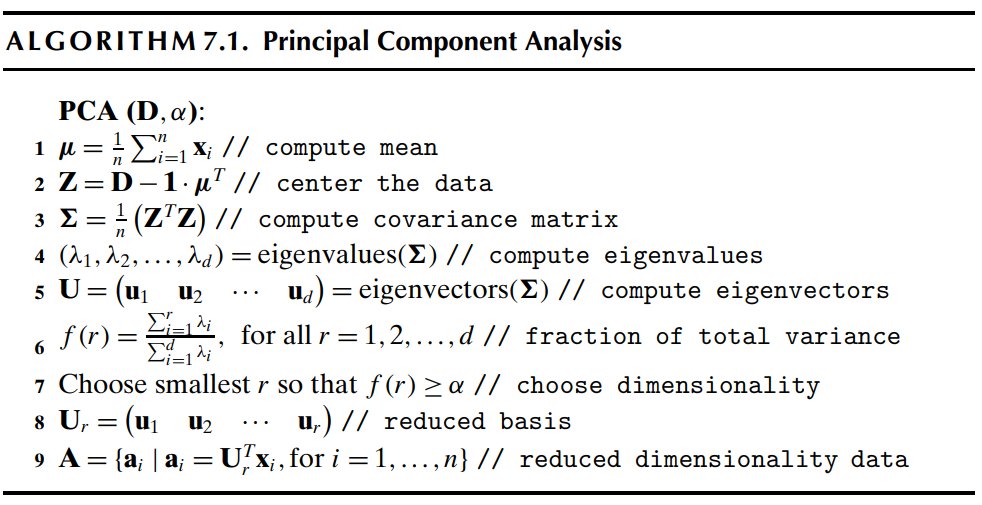
\includegraphics{../res/pca.PNG}

    \begin{tcolorbox}[breakable, size=fbox, boxrule=1pt, pad at break*=1mm,colback=cellbackground, colframe=cellborder]
\prompt{In}{incolor}{4}{\boxspacing}
\begin{Verbatim}[commandchars=\\\{\}]
\PY{k}{def} \PY{n+nf}{pca1}\PY{p}{(}\PY{n}{data}\PY{p}{:} \PY{n}{Tensor}\PY{p}{,} \PY{n}{alpha}\PY{p}{:} \PY{n+nb}{float}\PY{p}{)} \PY{o}{\PYZhy{}}\PY{o}{\PYZgt{}} \PY{n}{Tensor}\PY{p}{:}
    \PY{n}{centered\PYZus{}data}\PY{p}{:} \PY{n}{Tensor} \PY{o}{=} \PY{n}{data} \PY{o}{\PYZhy{}} \PY{n}{data}\PY{o}{.}\PY{n}{mean}\PY{p}{(}\PY{l+m+mi}{0}\PY{p}{)}
    \PY{n}{covariance}\PY{p}{:} \PY{n}{Tensor} \PY{o}{=} \PY{l+m+mi}{1} \PY{o}{/} \PY{n+nb}{len}\PY{p}{(}\PY{n}{data}\PY{p}{)} \PY{o}{*} \PY{n}{centered\PYZus{}data}\PY{o}{.}\PY{n}{T} \PY{o}{@} \PY{n}{centered\PYZus{}data}

    \PY{n}{eigen\PYZus{}values}\PY{p}{,} \PY{n}{eigen\PYZus{}vectors} \PY{o}{=} \PY{n}{linalg}\PY{o}{.}\PY{n}{eigh}\PY{p}{(}\PY{n}{covariance}\PY{p}{)}

    \PY{n}{variance}\PY{p}{:} \PY{n+nb}{float} \PY{o}{=} \PY{n}{covariance}\PY{o}{.}\PY{n}{trace}\PY{p}{(}\PY{p}{)}\PY{o}{.}\PY{n}{numpy}\PY{p}{(}\PY{p}{)}
    \PY{n}{projected\PYZus{}variance} \PY{o}{=} \PY{l+m+mf}{0.0}

    \PY{n}{i} \PY{o}{=} \PY{n+nb}{len}\PY{p}{(}\PY{n}{eigen\PYZus{}values}\PY{p}{)} \PY{o}{\PYZhy{}} \PY{l+m+mi}{1}
    \PY{k}{while} \PY{n}{i} \PY{o}{\PYZgt{}}\PY{o}{=} \PY{l+m+mi}{0} \PY{o+ow}{and} \PY{n}{projected\PYZus{}variance} \PY{o}{\PYZlt{}} \PY{n}{alpha} \PY{o}{*} \PY{n}{variance}\PY{p}{:}
        \PY{n}{projected\PYZus{}variance} \PY{o}{+}\PY{o}{=} \PY{n}{eigen\PYZus{}values}\PY{p}{[}\PY{n}{i}\PY{p}{]}
        \PY{n}{i} \PY{o}{\PYZhy{}}\PY{o}{=} \PY{l+m+mi}{1}

    \PY{n}{eigen\PYZus{}vectors} \PY{o}{=} \PY{n}{torch}\PY{o}{.}\PY{n}{fliplr}\PY{p}{(}\PY{n}{eigen\PYZus{}vectors}\PY{p}{[}\PY{p}{:}\PY{p}{,} \PY{n}{i} \PY{o}{+} \PY{l+m+mi}{1}\PY{p}{:}\PY{p}{]}\PY{p}{)}

    \PY{k}{return} \PY{n}{data} \PY{o}{@} \PY{n}{eigen\PYZus{}vectors}
\end{Verbatim}
\end{tcolorbox}

    \begin{tcolorbox}[breakable, size=fbox, boxrule=1pt, pad at break*=1mm,colback=cellbackground, colframe=cellborder]
\prompt{In}{incolor}{5}{\boxspacing}
\begin{Verbatim}[commandchars=\\\{\}]
\PY{c+c1}{\PYZsh{} pca1(training\PYZus{}data, 0.8)}
\end{Verbatim}
\end{tcolorbox}
\clearpage

    \subsection{Enhanced PCA algorithm}\label{enhanced-pca-algorithm}

Running Time: \(O(n^3)\) to calculate the eigen values and eigen vectors
of \(\frac{1}n\mathbf{X}_{n \times d}\mathbf{X}_{d\times n}^T\) matrix\\
Reference: Section 12.1.4 from C. M. Bishop, Pattern Recognition and
Machine Learning

    \begin{tcolorbox}[breakable, size=fbox, boxrule=1pt, pad at break*=1mm,colback=cellbackground, colframe=cellborder]
\prompt{In}{incolor}{6}{\boxspacing}
\begin{Verbatim}[commandchars=\\\{\}]
\PY{k}{def} \PY{n+nf}{pca2}\PY{p}{(}\PY{n}{data}\PY{p}{:} \PY{n}{Tensor}\PY{p}{,} \PY{n}{alpha}\PY{p}{:} \PY{n+nb}{float}\PY{p}{)} \PY{o}{\PYZhy{}}\PY{o}{\PYZgt{}} \PY{n}{Tensor}\PY{p}{:}
    \PY{n}{centered\PYZus{}data} \PY{o}{=} \PY{n}{data} \PY{o}{\PYZhy{}} \PY{n}{data}\PY{o}{.}\PY{n}{mean}\PY{p}{(}\PY{l+m+mi}{0}\PY{p}{)}

    \PY{n}{eigen\PYZus{}values}\PY{p}{,} \PY{n}{eigen\PYZus{}vectors} \PY{o}{=} \PY{n}{torch}\PY{o}{.}\PY{n}{linalg}\PY{o}{.}\PY{n}{eig}\PY{p}{(}\PY{l+m+mi}{1} \PY{o}{/} \PY{n+nb}{len}\PY{p}{(}\PY{n}{data}\PY{p}{)} \PY{o}{*} \PY{n}{centered\PYZus{}data} \PY{o}{@} \PY{n}{centered\PYZus{}data}\PY{o}{.}\PY{n}{T}\PY{p}{)}
    \PY{n}{eigen\PYZus{}values} \PY{o}{=} \PY{n}{eigen\PYZus{}values}\PY{o}{.}\PY{n}{real}
    \PY{n}{eigen\PYZus{}vectors} \PY{o}{=} \PY{n}{eigen\PYZus{}vectors}\PY{o}{.}\PY{n}{real}

    \PY{n}{variance}\PY{p}{:} \PY{n+nb}{float} \PY{o}{=} \PY{p}{(}\PY{l+m+mi}{1} \PY{o}{/} \PY{n+nb}{len}\PY{p}{(}\PY{n}{data}\PY{p}{)} \PY{o}{*} \PY{n}{centered\PYZus{}data}\PY{o}{.}\PY{n}{T} \PY{o}{@} \PY{n}{centered\PYZus{}data}\PY{p}{)}\PY{o}{.}\PY{n}{trace}\PY{p}{(}\PY{p}{)}\PY{o}{.}\PY{n}{numpy}\PY{p}{(}\PY{p}{)}
    \PY{n}{projected\PYZus{}variance} \PY{o}{=} \PY{l+m+mf}{0.0}

    \PY{n}{idxs} \PY{o}{=} \PY{n}{torch}\PY{o}{.}\PY{n}{argsort}\PY{p}{(}\PY{n}{eigen\PYZus{}values}\PY{p}{,} \PY{n}{descending}\PY{o}{=}\PY{k+kc}{True}\PY{p}{)}
    \PY{n}{eigen\PYZus{}values} \PY{o}{=} \PY{n}{eigen\PYZus{}values}\PY{p}{[}\PY{n}{idxs}\PY{p}{]}
    \PY{n}{eigen\PYZus{}vectors} \PY{o}{=} \PY{n}{eigen\PYZus{}vectors}\PY{p}{[}\PY{p}{:}\PY{p}{,} \PY{n}{idxs}\PY{p}{]}

    \PY{n}{i} \PY{o}{=} \PY{l+m+mi}{0}
    \PY{k}{while} \PY{n}{i} \PY{o}{\PYZlt{}} \PY{n+nb}{len}\PY{p}{(}\PY{n}{eigen\PYZus{}values}\PY{p}{)} \PY{o+ow}{and} \PY{n}{projected\PYZus{}variance} \PY{o}{\PYZlt{}} \PY{n}{alpha} \PY{o}{*} \PY{n}{variance}\PY{p}{:}
        \PY{n}{projected\PYZus{}variance} \PY{o}{+}\PY{o}{=} \PY{n}{eigen\PYZus{}values}\PY{p}{[}\PY{n}{i}\PY{p}{]}
        \PY{n}{i} \PY{o}{+}\PY{o}{=} \PY{l+m+mi}{1}

    \PY{n}{new\PYZus{}basis} \PY{o}{=} \PY{n}{centered\PYZus{}data}\PY{o}{.}\PY{n}{T} \PY{o}{@} \PY{n}{eigen\PYZus{}vectors}
    \PY{n}{new\PYZus{}basis} \PY{o}{/}\PY{o}{=} \PY{n}{torch}\PY{o}{.}\PY{n}{sqrt}\PY{p}{(}\PY{n}{eigen\PYZus{}values} \PY{o}{*} \PY{n+nb}{len}\PY{p}{(}\PY{n}{data}\PY{p}{)}\PY{p}{)}

    \PY{n}{new\PYZus{}basis} \PY{o}{=} \PY{n}{new\PYZus{}basis}\PY{p}{[}\PY{p}{:}\PY{p}{,} \PY{p}{:}\PY{n}{i}\PY{p}{]}

    \PY{k}{return} \PY{n}{new\PYZus{}basis}
\end{Verbatim}
\end{tcolorbox}

    \begin{tcolorbox}[breakable, size=fbox, boxrule=1pt, pad at break*=1mm,colback=cellbackground, colframe=cellborder]
\prompt{In}{incolor}{7}{\boxspacing}
\begin{Verbatim}[commandchars=\\\{\}]
\PY{n}{alpha} \PY{o}{=} \PY{l+m+mf}{0.95}

\PY{n}{new\PYZus{}basis} \PY{o}{=} \PY{n}{pca2}\PY{p}{(}\PY{n}{training\PYZus{}data}\PY{p}{,} \PY{n}{alpha}\PY{p}{)}

\PY{c+c1}{\PYZsh{} project training data}
\PY{n}{projected\PYZus{}training\PYZus{}data} \PY{o}{=} \PY{n}{training\PYZus{}data} \PY{o}{@} \PY{n}{new\PYZus{}basis}
\end{Verbatim}
\end{tcolorbox}

    Classify test data using KNN

    \begin{tcolorbox}[breakable, size=fbox, boxrule=1pt, pad at break*=1mm,colback=cellbackground, colframe=cellborder]
\prompt{In}{incolor}{4}{\boxspacing}
\begin{Verbatim}[commandchars=\\\{\}]
\PY{k}{def} \PY{n+nf}{knn}\PY{p}{(}\PY{n}{test\PYZus{}data}\PY{p}{:} \PY{n}{Tensor}\PY{p}{,} \PY{n}{training\PYZus{}data}\PY{p}{:} \PY{n}{Tensor}\PY{p}{,} \PY{n}{k}\PY{p}{:} \PY{n+nb}{int}\PY{p}{)}\PY{p}{:}
    \PY{n}{distance\PYZus{}matrix} \PY{o}{=} \PY{n}{torch}\PY{o}{.}\PY{n}{cdist}\PY{p}{(}\PY{n}{test\PYZus{}data}\PY{p}{,} \PY{n}{training\PYZus{}data}\PY{p}{)}
    \PY{n}{indices} \PY{o}{=} \PY{n}{torch}\PY{o}{.}\PY{n}{argsort}\PY{p}{(}\PY{n}{distance\PYZus{}matrix}\PY{p}{,} \PY{n}{dim}\PY{o}{=}\PY{l+m+mi}{1}\PY{p}{)}
    \PY{k}{return} \PY{n}{indices}\PY{p}{[}\PY{p}{:}\PY{p}{,} \PY{p}{:}\PY{n}{k}\PY{p}{]}
\end{Verbatim}
\end{tcolorbox}

    \begin{tcolorbox}[breakable, size=fbox, boxrule=1pt, pad at break*=1mm,colback=cellbackground, colframe=cellborder]
\prompt{In}{incolor}{25}{\boxspacing}
\begin{Verbatim}[commandchars=\\\{\}]
\PY{n}{result\PYZus{}labels} \PY{o}{=} \PY{n}{training\PYZus{}labels}\PY{p}{[}\PY{n}{knn}\PY{p}{(}\PY{n}{test\PYZus{}data} \PY{o}{@} \PY{n}{new\PYZus{}basis}\PY{p}{,} \PY{n}{projected\PYZus{}training\PYZus{}data}\PY{p}{,} \PY{l+m+mi}{1}\PY{p}{)}\PY{p}{]}\PY{o}{.}\PY{n}{mode}\PY{p}{(}\PY{n}{keepdim}\PY{o}{=}\PY{k+kc}{True}\PY{p}{)}\PY{p}{[}\PY{l+m+mi}{0}\PY{p}{]}
\end{Verbatim}
\end{tcolorbox}

    \begin{Verbatim}[commandchars=\\\{\}]
tensor(6272.0381)
    \end{Verbatim}

    \begin{tcolorbox}[breakable, size=fbox, boxrule=1pt, pad at break*=1mm,colback=cellbackground, colframe=cellborder]
\prompt{In}{incolor}{10}{\boxspacing}
\begin{Verbatim}[commandchars=\\\{\}]
\PY{n}{Latex}\PY{p}{(}\PY{l+s+sa}{rf}\PY{l+s+s2}{\PYZdq{}}\PY{l+s+s2}{for \PYZdl{}}\PY{l+s+s2}{\PYZbs{}}\PY{l+s+s2}{alpha\PYZdl{} = }\PY{l+s+si}{\PYZob{}}\PY{n}{alpha}\PY{l+s+si}{\PYZcb{}}\PY{l+s+s2}{, accuracy = }\PY{l+s+si}{\PYZob{}}\PY{l+m+mi}{1}\PY{+w}{ }\PY{o}{\PYZhy{}}\PY{+w}{ }\PY{n}{torch}\PY{o}{.}\PY{n}{count\PYZus{}nonzero}\PY{p}{(}\PY{n}{result\PYZus{}labels}\PY{+w}{ }\PY{o}{\PYZhy{}}\PY{+w}{ }\PY{n}{test\PYZus{}labels}\PY{p}{[}\PY{p}{:}\PY{p}{,}\PY{+w}{ }\PY{k+kc}{None}\PY{p}{]}\PY{p}{)}\PY{+w}{ }\PY{o}{/}\PY{+w}{ }\PY{n+nb}{len}\PY{p}{(}\PY{n}{result\PYZus{}labels}\PY{p}{)}\PY{l+s+si}{\PYZcb{}}\PY{l+s+s2}{\PYZdq{}}\PY{p}{)}
\end{Verbatim}
\end{tcolorbox}
 
            
\prompt{Out}{outcolor}{10}{}
    
    for $\alpha$ = 0.95, accuracy = 0.935

    

    \begin{tcolorbox}[breakable, size=fbox, boxrule=1pt, pad at break*=1mm,colback=cellbackground, colframe=cellborder]
\prompt{In}{incolor}{44}{\boxspacing}
\begin{Verbatim}[commandchars=\\\{\}]
\PY{k}{def} \PY{n+nf}{pca\PYZus{}classify}\PY{p}{(}\PY{n}{training\PYZus{}data}\PY{p}{:} \PY{n}{Tensor}\PY{p}{,} \PY{n}{test\PYZus{}data}\PY{p}{:} \PY{n}{Tensor}\PY{p}{,} \PY{n}{training\PYZus{}labels}\PY{p}{:} \PY{n}{Tensor}\PY{p}{,} \PY{n}{test\PYZus{}labels}\PY{p}{:} \PY{n}{Tensor}\PY{p}{,} \PY{n}{alpha}\PY{p}{:} \PY{n+nb}{float}\PY{p}{,} \PY{n}{k}\PY{p}{:} \PY{n+nb}{int}\PY{p}{)} \PY{o}{\PYZhy{}}\PY{o}{\PYZgt{}} \PY{n+nb}{float}\PY{p}{:}
    \PY{n}{new\PYZus{}basis} \PY{o}{=} \PY{n}{pca2}\PY{p}{(}\PY{n}{training\PYZus{}data}\PY{p}{,} \PY{n}{alpha}\PY{p}{)}
    \PY{n}{projected\PYZus{}training\PYZus{}data} \PY{o}{=} \PY{n}{training\PYZus{}data} \PY{o}{@} \PY{n}{new\PYZus{}basis}
    \PY{n}{result\PYZus{}labels} \PY{o}{=} \PY{n}{training\PYZus{}labels}\PY{p}{[}\PY{n}{knn}\PY{p}{(}\PY{n}{test\PYZus{}data} \PY{o}{@} \PY{n}{new\PYZus{}basis}\PY{p}{,} \PY{n}{projected\PYZus{}training\PYZus{}data}\PY{p}{,} \PY{n}{k}\PY{p}{)}\PY{p}{]}\PY{o}{.}\PY{n}{mode}\PY{p}{(}\PY{n}{keepdim}\PY{o}{=}\PY{k+kc}{True}\PY{p}{)}\PY{p}{[}\PY{l+m+mi}{0}\PY{p}{]}
    \PY{k}{return} \PY{l+m+mi}{1} \PY{o}{\PYZhy{}} \PY{n}{torch}\PY{o}{.}\PY{n}{count\PYZus{}nonzero}\PY{p}{(}\PY{n}{result\PYZus{}labels} \PY{o}{\PYZhy{}} \PY{n}{test\PYZus{}labels}\PY{p}{[}\PY{p}{:}\PY{p}{,} \PY{k+kc}{None}\PY{p}{]}\PY{p}{)} \PY{o}{/} \PY{n+nb}{len}\PY{p}{(}\PY{n}{result\PYZus{}labels}\PY{p}{)}
\end{Verbatim}
\end{tcolorbox}

    \begin{tcolorbox}[breakable, size=fbox, boxrule=1pt, pad at break*=1mm,colback=cellbackground, colframe=cellborder]
\prompt{In}{incolor}{12}{\boxspacing}
\begin{Verbatim}[commandchars=\\\{\}]
\PY{n}{alpha} \PY{o}{=} \PY{l+m+mf}{0.8}
\PY{n}{accuracy} \PY{o}{=} \PY{n}{pca\PYZus{}classify}\PY{p}{(}\PY{n}{training\PYZus{}data}\PY{p}{,} \PY{n}{test\PYZus{}data}\PY{p}{,} \PY{n}{training\PYZus{}labels}\PY{p}{,} \PY{n}{test\PYZus{}labels}\PY{p}{,} \PY{n}{alpha}\PY{p}{,} \PY{l+m+mi}{1}\PY{p}{)}
\PY{n}{Latex}\PY{p}{(}\PY{l+s+sa}{rf}\PY{l+s+s2}{\PYZdq{}}\PY{l+s+s2}{for \PYZdl{}}\PY{l+s+s2}{\PYZbs{}}\PY{l+s+s2}{alpha\PYZdl{} = }\PY{l+s+si}{\PYZob{}}\PY{n}{alpha}\PY{l+s+si}{\PYZcb{}}\PY{l+s+s2}{, accuracy = }\PY{l+s+si}{\PYZob{}}\PY{n}{accuracy}\PY{l+s+si}{\PYZcb{}}\PY{l+s+s2}{\PYZdq{}}\PY{p}{)}
\end{Verbatim}
\end{tcolorbox}
 
            
\prompt{Out}{outcolor}{12}{}
    
    for $\alpha$ = 0.8, accuracy = 0.9299999999999999

    

    \begin{tcolorbox}[breakable, size=fbox, boxrule=1pt, pad at break*=1mm,colback=cellbackground, colframe=cellborder]
\prompt{In}{incolor}{13}{\boxspacing}
\begin{Verbatim}[commandchars=\\\{\}]
\PY{n}{alpha} \PY{o}{=} \PY{l+m+mf}{0.85}
\PY{n}{accuracy} \PY{o}{=} \PY{n}{pca\PYZus{}classify}\PY{p}{(}\PY{n}{training\PYZus{}data}\PY{p}{,} \PY{n}{test\PYZus{}data}\PY{p}{,} \PY{n}{training\PYZus{}labels}\PY{p}{,} \PY{n}{test\PYZus{}labels}\PY{p}{,} \PY{n}{alpha}\PY{p}{,} \PY{l+m+mi}{1}\PY{p}{)}
\PY{n}{Latex}\PY{p}{(}\PY{l+s+sa}{rf}\PY{l+s+s2}{\PYZdq{}}\PY{l+s+s2}{for \PYZdl{}}\PY{l+s+s2}{\PYZbs{}}\PY{l+s+s2}{alpha\PYZdl{} = }\PY{l+s+si}{\PYZob{}}\PY{n}{alpha}\PY{l+s+si}{\PYZcb{}}\PY{l+s+s2}{, accuracy = }\PY{l+s+si}{\PYZob{}}\PY{n}{accuracy}\PY{l+s+si}{\PYZcb{}}\PY{l+s+s2}{\PYZdq{}}\PY{p}{)}
\end{Verbatim}
\end{tcolorbox}
 
            
\prompt{Out}{outcolor}{13}{}
    
    for $\alpha$ = 0.85, accuracy = 0.94

    

    \begin{tcolorbox}[breakable, size=fbox, boxrule=1pt, pad at break*=1mm,colback=cellbackground, colframe=cellborder]
\prompt{In}{incolor}{14}{\boxspacing}
\begin{Verbatim}[commandchars=\\\{\}]
\PY{n}{alpha} \PY{o}{=} \PY{l+m+mf}{0.9}
\PY{n}{accuracy} \PY{o}{=} \PY{n}{pca\PYZus{}classify}\PY{p}{(}\PY{n}{training\PYZus{}data}\PY{p}{,} \PY{n}{test\PYZus{}data}\PY{p}{,} \PY{n}{training\PYZus{}labels}\PY{p}{,} \PY{n}{test\PYZus{}labels}\PY{p}{,} \PY{n}{alpha}\PY{p}{,} \PY{l+m+mi}{1}\PY{p}{)}
\PY{n}{Latex}\PY{p}{(}\PY{l+s+sa}{rf}\PY{l+s+s2}{\PYZdq{}}\PY{l+s+s2}{for \PYZdl{}}\PY{l+s+s2}{\PYZbs{}}\PY{l+s+s2}{alpha\PYZdl{} = }\PY{l+s+si}{\PYZob{}}\PY{n}{alpha}\PY{l+s+si}{\PYZcb{}}\PY{l+s+s2}{, accuracy = }\PY{l+s+si}{\PYZob{}}\PY{n}{accuracy}\PY{l+s+si}{\PYZcb{}}\PY{l+s+s2}{\PYZdq{}}\PY{p}{)}
\end{Verbatim}
\end{tcolorbox}
 
            
\prompt{Out}{outcolor}{14}{}
    
    for $\alpha$ = 0.9, accuracy = 0.945

    

    \begin{tcolorbox}[breakable, size=fbox, boxrule=1pt, pad at break*=1mm,colback=cellbackground, colframe=cellborder]
\prompt{In}{incolor}{15}{\boxspacing}
\begin{Verbatim}[commandchars=\\\{\}]
\PY{n}{alpha} \PY{o}{=} \PY{l+m+mf}{0.95}
\PY{n}{accuracy} \PY{o}{=} \PY{n}{pca\PYZus{}classify}\PY{p}{(}\PY{n}{training\PYZus{}data}\PY{p}{,} \PY{n}{test\PYZus{}data}\PY{p}{,} \PY{n}{training\PYZus{}labels}\PY{p}{,} \PY{n}{test\PYZus{}labels}\PY{p}{,} \PY{n}{alpha}\PY{p}{,} \PY{l+m+mi}{1}\PY{p}{)}
\PY{n}{Latex}\PY{p}{(}\PY{l+s+sa}{rf}\PY{l+s+s2}{\PYZdq{}}\PY{l+s+s2}{for \PYZdl{}}\PY{l+s+s2}{\PYZbs{}}\PY{l+s+s2}{alpha\PYZdl{} = }\PY{l+s+si}{\PYZob{}}\PY{n}{alpha}\PY{l+s+si}{\PYZcb{}}\PY{l+s+s2}{, accuracy = }\PY{l+s+si}{\PYZob{}}\PY{n}{accuracy}\PY{l+s+si}{\PYZcb{}}\PY{l+s+s2}{\PYZdq{}}\PY{p}{)}
\end{Verbatim}
\end{tcolorbox}
 
            
\prompt{Out}{outcolor}{15}{}
    
    for $\alpha$ = 0.95, accuracy = 0.935

    

    It is clear that the accuracy increases by increasing \(\alpha\)
(\(\alpha \propto\) accuracy).\\
However, the accuracy seems to decreases as \(\alpha\) goes from 0.9 to
0.95

    \section{Classification using LDA}\label{classification-using-lda}

\subsection{Original LDA Algorithm}\label{original-lda-algorithm}

Running Time: \(O(d^3)\) to calculate the eigen values and eigen vectors
of \(\Sigma_{d \times d}\) matrix\\
\strut \\
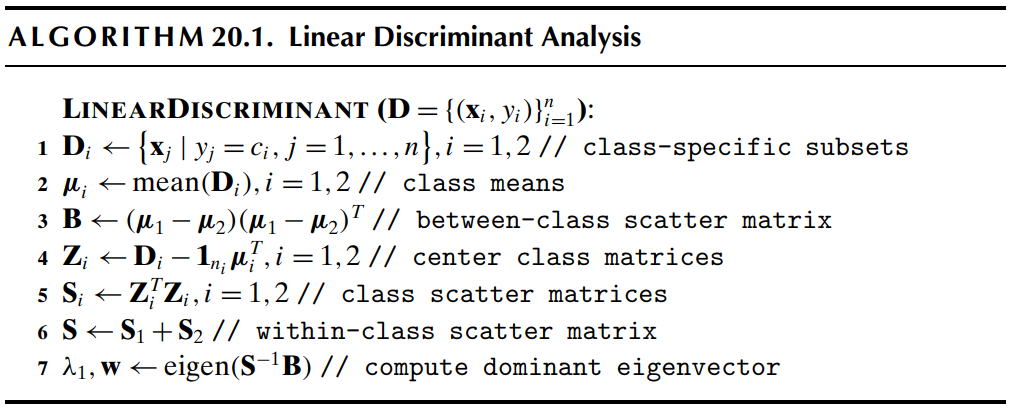
\includegraphics{../res/lda.PNG}

    \begin{tcolorbox}[breakable, size=fbox, boxrule=1pt, pad at break*=1mm,colback=cellbackground, colframe=cellborder]
\prompt{In}{incolor}{5}{\boxspacing}
\begin{Verbatim}[commandchars=\\\{\}]
\PY{k}{def} \PY{n+nf}{LDA}\PY{p}{(}\PY{n}{D} \PY{p}{,} \PY{n}{y}\PY{p}{)}\PY{p}{:}
    \PY{n}{n\PYZus{}features} \PY{o}{=} \PY{n+nb}{len}\PY{p}{(}\PY{n}{D}\PY{p}{[}\PY{l+m+mi}{0}\PY{p}{]}\PY{p}{)}
    \PY{n}{classes} \PY{o}{=} \PY{n}{torch}\PY{o}{.}\PY{n}{unique}\PY{p}{(}\PY{n}{y}\PY{p}{)}
    \PY{n}{n\PYZus{}classes} \PY{o}{=} \PY{n+nb}{len}\PY{p}{(}\PY{n}{classes}\PY{p}{)}

    \PY{n}{overall\PYZus{}mean} \PY{o}{=} \PY{n}{torch}\PY{o}{.}\PY{n}{mean}\PY{p}{(}\PY{n}{D} \PY{p}{,}\PY{n}{dim}\PY{o}{=}\PY{l+m+mi}{0}\PY{p}{)}

    \PY{c+c1}{\PYZsh{} between\PYZhy{}class scatter}
    \PY{n}{Sb} \PY{o}{=} \PY{n}{torch}\PY{o}{.}\PY{n}{zeros}\PY{p}{(}\PY{p}{(}\PY{n}{n\PYZus{}features} \PY{p}{,} \PY{n}{n\PYZus{}features}\PY{p}{)}\PY{p}{)}

    \PY{c+c1}{\PYZsh{} within\PYZhy{}class scatter}
    \PY{n}{S} \PY{o}{=} \PY{n}{torch}\PY{o}{.}\PY{n}{zeros}\PY{p}{(}\PY{p}{(}\PY{n}{n\PYZus{}features} \PY{p}{,} \PY{n}{n\PYZus{}features}\PY{p}{)}\PY{p}{)}

    \PY{k}{for} \PY{n}{i} \PY{o+ow}{in} \PY{n}{classes}\PY{p}{:}
        \PY{n}{Kth\PYZus{}class} \PY{o}{=} \PY{n}{D}\PY{p}{[}\PY{n}{y} \PY{o}{==} \PY{n}{i}\PY{p}{]}
        \PY{n}{cur\PYZus{}mean} \PY{o}{=} \PY{n}{torch}\PY{o}{.}\PY{n}{mean}\PY{p}{(}\PY{n}{Kth\PYZus{}class} \PY{p}{,} \PY{n}{dim}\PY{o}{=}\PY{l+m+mi}{0}\PY{p}{)}
       
        \PY{c+c1}{\PYZsh{} calculate between class scatter matrix}
        \PY{n}{centered\PYZus{}kth\PYZus{}mean} \PY{o}{=} \PY{p}{(}\PY{n}{cur\PYZus{}mean} \PY{o}{\PYZhy{}} \PY{n}{overall\PYZus{}mean}\PY{p}{)}\PY{o}{.}\PY{n}{unsqueeze}\PY{p}{(}\PY{l+m+mi}{1}\PY{p}{)}
        \PY{n}{Sb} \PY{o}{+}\PY{o}{=} \PY{p}{(}\PY{n}{Kth\PYZus{}class}\PY{o}{.}\PY{n}{shape}\PY{p}{[}\PY{l+m+mi}{0}\PY{p}{]} \PY{o}{*} \PY{n}{Tensor}\PY{o}{.}\PY{n}{matmul}\PY{p}{(}\PY{n}{centered\PYZus{}kth\PYZus{}mean}\PY{p}{,}\PY{n}{centered\PYZus{}kth\PYZus{}mean}\PY{o}{.}\PY{n}{T}\PY{p}{)}\PY{p}{)}

        \PY{c+c1}{\PYZsh{} calculate within class scatter matrix}
        \PY{n}{centered\PYZus{}kth\PYZus{}class} \PY{o}{=} \PY{n}{Kth\PYZus{}class} \PY{o}{\PYZhy{}} \PY{n}{cur\PYZus{}mean}
        \PY{n}{S} \PY{o}{+}\PY{o}{=} \PY{n}{Tensor}\PY{o}{.}\PY{n}{matmul}\PY{p}{(}\PY{n}{centered\PYZus{}kth\PYZus{}class}\PY{o}{.}\PY{n}{T}\PY{p}{,}\PY{n}{centered\PYZus{}kth\PYZus{}class}\PY{p}{)}


    \PY{c+c1}{\PYZsh{}compute matrix (S\PYZca{}\PYZhy{}1*B) }
    \PY{n}{A} \PY{o}{=} \PY{n}{linalg}\PY{o}{.}\PY{n}{pinv}\PY{p}{(}\PY{n}{S}\PY{p}{)} \PY{o}{@} \PY{n}{Sb}
    
    \PY{c+c1}{\PYZsh{}Compute the eignValues and eignVectors}
    \PY{n}{eigenvalues}\PY{p}{,} \PY{n}{eigenvectors} \PY{o}{=} \PY{n}{linalg}\PY{o}{.}\PY{n}{eig}\PY{p}{(}\PY{n}{A}\PY{p}{)}
    \PY{n}{eigenvalues}\PY{p}{,} \PY{n}{eigenvectors} \PY{o}{=}\PY{n}{eigenvalues}\PY{o}{.}\PY{n}{real}\PY{p}{,} \PY{n}{eigenvectors}\PY{o}{.}\PY{n}{real}
    
    \PY{c+c1}{\PYZsh{}Sort the eignValues and eignVectors}
    \PY{n}{idxs} \PY{o}{=} \PY{n}{torch}\PY{o}{.}\PY{n}{argsort}\PY{p}{(}\PY{n}{eigenvalues}\PY{p}{,}\PY{n}{descending}\PY{o}{=}\PY{k+kc}{True}\PY{p}{)}
    \PY{n}{eigenvectors} \PY{o}{=} \PY{n}{eigenvectors}\PY{p}{[}\PY{p}{:}\PY{p}{,}\PY{n}{idxs}\PY{p}{]}

    \PY{k}{return} \PY{n}{eigenvectors}\PY{p}{[}\PY{p}{:}\PY{p}{,}\PY{p}{:}\PY{n}{n\PYZus{}classes}\PY{o}{\PYZhy{}}\PY{l+m+mi}{1}\PY{p}{]}
\end{Verbatim}
\end{tcolorbox}

    \begin{tcolorbox}[breakable, size=fbox, boxrule=1pt, pad at break*=1mm,colback=cellbackground, colframe=cellborder]
\prompt{In}{incolor}{6}{\boxspacing}
\begin{Verbatim}[commandchars=\\\{\}]
\PY{k}{def} \PY{n+nf}{lda\PYZus{}classify}\PY{p}{(}\PY{n}{training\PYZus{}data}\PY{p}{,} \PY{n}{test\PYZus{}data}\PY{p}{,} \PY{n}{training\PYZus{}labels}\PY{p}{,} \PY{n}{test\PYZus{}labels}\PY{p}{,} \PY{n}{k}\PY{p}{)}\PY{p}{:}
    \PY{n}{projection\PYZus{}matrix} \PY{o}{=} \PY{n}{LDA}\PY{p}{(}\PY{n}{training\PYZus{}data}\PY{p}{,}\PY{n}{training\PYZus{}labels}\PY{p}{)} 
    \PY{n}{projected\PYZus{}training\PYZus{}matrix} \PY{o}{=} \PY{n}{training\PYZus{}data} \PY{o}{@} \PY{n}{projection\PYZus{}matrix}
    \PY{n}{projected\PYZus{}test\PYZus{}matrix} \PY{o}{=} \PY{n}{test\PYZus{}data} \PY{o}{@} \PY{n}{projection\PYZus{}matrix}
    
    \PY{n}{result\PYZus{}labels} \PY{o}{=} \PY{n}{training\PYZus{}labels}\PY{p}{[}\PY{n}{knn}\PY{p}{(}\PY{n}{projected\PYZus{}test\PYZus{}matrix}\PY{p}{,}\PY{n}{projected\PYZus{}training\PYZus{}matrix}\PY{p}{,} \PY{n}{k}\PY{p}{)}\PY{p}{]}\PY{o}{.}\PY{n}{mode}\PY{p}{(}\PY{n}{keepdim}\PY{o}{=}\PY{k+kc}{True}\PY{p}{)}\PY{p}{[}\PY{l+m+mi}{0}\PY{p}{]}
    \PY{k}{return} \PY{l+m+mi}{1} \PY{o}{\PYZhy{}} \PY{n}{torch}\PY{o}{.}\PY{n}{count\PYZus{}nonzero}\PY{p}{(}\PY{n}{result\PYZus{}labels} \PY{o}{\PYZhy{}} \PY{n}{test\PYZus{}labels}\PY{p}{[}\PY{p}{:}\PY{p}{,} \PY{k+kc}{None}\PY{p}{]}\PY{p}{)} \PY{o}{/} \PY{n+nb}{len}\PY{p}{(}\PY{n}{result\PYZus{}labels}\PY{p}{)}
\end{Verbatim}
\end{tcolorbox}

    \begin{tcolorbox}[breakable, size=fbox, boxrule=1pt, pad at break*=1mm,colback=cellbackground, colframe=cellborder]
\prompt{In}{incolor}{7}{\boxspacing}
\begin{Verbatim}[commandchars=\\\{\}]
\PY{n}{k} \PY{o}{=} \PY{l+m+mi}{1}

\PY{n}{accuracy} \PY{o}{=} \PY{n}{lda\PYZus{}classify}\PY{p}{(}\PY{n}{training\PYZus{}data}\PY{p}{,} \PY{n}{test\PYZus{}data}\PY{p}{,} \PY{n}{training\PYZus{}labels}\PY{p}{,} \PY{n}{test\PYZus{}labels}\PY{p}{,} \PY{n}{k}\PY{p}{)}
\PY{n+nb}{print}\PY{p}{(}\PY{l+s+sa}{f}\PY{l+s+s2}{\PYZdq{}}\PY{l+s+s2}{accuracy = }\PY{l+s+si}{\PYZob{}}\PY{n}{accuracy}\PY{l+s+si}{\PYZcb{}}\PY{l+s+s2}{\PYZdq{}}\PY{p}{)}
\end{Verbatim}
\end{tcolorbox}

    \begin{Verbatim}[commandchars=\\\{\}]
accuracy = 0.96
    \end{Verbatim}

\clearpage

    \section{Classifier Tuning}\label{classifier-tuning}

\subsection{\texorpdfstring{PCA using \(\alpha\) =
0.9}{PCA using \textbackslash alpha = 0.9}}\label{pca-using-alpha-0.9}

    \begin{tcolorbox}[breakable, size=fbox, boxrule=1pt, pad at break*=1mm,colback=cellbackground, colframe=cellborder]
\prompt{In}{incolor}{16}{\boxspacing}
\begin{Verbatim}[commandchars=\\\{\}]
\PY{n}{ks} \PY{o}{=} \PY{p}{[}\PY{l+m+mi}{1}\PY{p}{,} \PY{l+m+mi}{3}\PY{p}{,} \PY{l+m+mi}{5}\PY{p}{,} \PY{l+m+mi}{7}\PY{p}{]}
\PY{n}{alpha} \PY{o}{=} \PY{l+m+mf}{0.9}

\PY{n}{accuracies} \PY{o}{=} \PY{p}{[}\PY{n}{pca\PYZus{}classify}\PY{p}{(}\PY{n}{training\PYZus{}data}\PY{p}{,} \PY{n}{test\PYZus{}data}\PY{p}{,} \PY{n}{training\PYZus{}labels}\PY{p}{,} \PY{n}{test\PYZus{}labels}\PY{p}{,} \PY{n}{alpha}\PY{p}{,} \PY{n}{k}\PY{p}{)} \PY{k}{for} \PY{n}{k} \PY{o+ow}{in} \PY{n}{ks}\PY{p}{]}
\PY{n}{plt}\PY{o}{.}\PY{n}{xlabel}\PY{p}{(}\PY{l+s+s2}{\PYZdq{}}\PY{l+s+s2}{k}\PY{l+s+s2}{\PYZdq{}}\PY{p}{)}
\PY{n}{plt}\PY{o}{.}\PY{n}{ylabel}\PY{p}{(}\PY{l+s+s2}{\PYZdq{}}\PY{l+s+s2}{accuracy}\PY{l+s+s2}{\PYZdq{}}\PY{p}{)}
\PY{n}{plt}\PY{o}{.}\PY{n}{scatter}\PY{p}{(}\PY{n}{ks}\PY{p}{,} \PY{n}{accuracies}\PY{p}{)}
\end{Verbatim}
\end{tcolorbox}

            \begin{tcolorbox}[breakable, size=fbox, boxrule=.5pt, pad at break*=1mm, opacityfill=0]
\prompt{Out}{outcolor}{16}{\boxspacing}
\begin{Verbatim}[commandchars=\\\{\}]
<matplotlib.collections.PathCollection at 0x1a51a12d110>
\end{Verbatim}
\end{tcolorbox}
        
    \begin{center}
    \adjustimage{max size={0.9\linewidth}{0.9\paperheight}}{pca_files/pca_26_1.png}
    \end{center}
    { \hspace*{\fill} \\}
    
    Using KNN classification with k = 1 gives the most accurate results

    \subsection{LDA}\label{lda}

    \begin{tcolorbox}[breakable, size=fbox, boxrule=1pt, pad at break*=1mm,colback=cellbackground, colframe=cellborder]
\prompt{In}{incolor}{ }{\boxspacing}
\begin{Verbatim}[commandchars=\\\{\}]
\PY{n}{ks} \PY{o}{=} \PY{p}{[}\PY{l+m+mi}{1}\PY{p}{,} \PY{l+m+mi}{3}\PY{p}{,} \PY{l+m+mi}{5}\PY{p}{,} \PY{l+m+mi}{7}\PY{p}{]}

\PY{n}{accuracies} \PY{o}{=} \PY{p}{[}\PY{n}{lda\PYZus{}classify}\PY{p}{(}\PY{n}{training\PYZus{}data}\PY{p}{,} \PY{n}{test\PYZus{}data}\PY{p}{,} \PY{n}{training\PYZus{}labels}\PY{p}{,} \PY{n}{test\PYZus{}labels}\PY{p}{,} \PY{n}{k}\PY{p}{)} \PY{k}{for} \PY{n}{k} \PY{o+ow}{in} \PY{n}{ks}\PY{p}{]}
\PY{n}{plt}\PY{o}{.}\PY{n}{xlabel}\PY{p}{(}\PY{l+s+s2}{\PYZdq{}}\PY{l+s+s2}{k}\PY{l+s+s2}{\PYZdq{}}\PY{p}{)}
\PY{n}{plt}\PY{o}{.}\PY{n}{ylabel}\PY{p}{(}\PY{l+s+s2}{\PYZdq{}}\PY{l+s+s2}{accuracy}\PY{l+s+s2}{\PYZdq{}}\PY{p}{)}
\PY{n}{plt}\PY{o}{.}\PY{n}{scatter}\PY{p}{(}\PY{n}{ks}\PY{p}{,} \PY{n}{accuracies}\PY{p}{)}
\end{Verbatim}
\end{tcolorbox}

    \begin{figure}
\centering
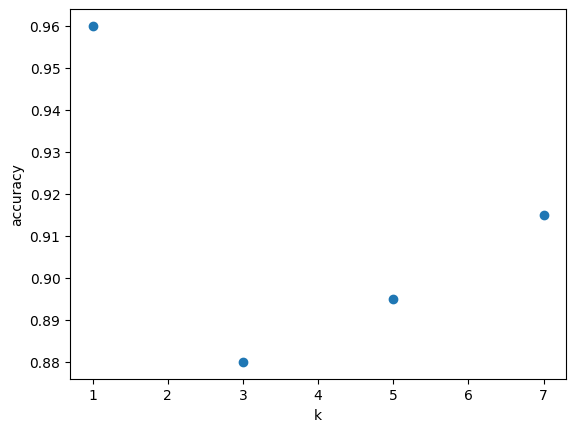
\includegraphics{../res/output.PNG}
\caption{pca}
\end{figure}

    Using KNN classification with k = 1 gives the most accurate results

\clearpage

    \section{Compare vs Non-Face Images}\label{compare-vs-non-face-images}

Read non-face data (iris dataset)

    \begin{tcolorbox}[breakable, size=fbox, boxrule=1pt, pad at break*=1mm,colback=cellbackground, colframe=cellborder]
\prompt{In}{incolor}{11}{\boxspacing}
\begin{Verbatim}[commandchars=\\\{\}]
\PY{n}{iris\PYZus{}path\PYZus{}1} \PY{o}{=} \PY{l+s+s2}{\PYZdq{}}\PY{l+s+s2}{../data/iris/iris\PYZhy{}setosa}\PY{l+s+s2}{\PYZdq{}}
\PY{n}{iris\PYZus{}path\PYZus{}2} \PY{o}{=} \PY{l+s+s2}{\PYZdq{}}\PY{l+s+s2}{../data/iris/iris\PYZhy{}versicolour}\PY{l+s+s2}{\PYZdq{}}
\PY{n}{iris\PYZus{}path\PYZus{}3} \PY{o}{=} \PY{l+s+s2}{\PYZdq{}}\PY{l+s+s2}{../data/iris/iris\PYZhy{}virginica}\PY{l+s+s2}{\PYZdq{}}

\PY{n}{iris\PYZus{}images} \PY{o}{=} \PY{p}{[}\PY{n}{Image}\PY{o}{.}\PY{n}{open}\PY{p}{(}\PY{l+s+sa}{f}\PY{l+s+s2}{\PYZdq{}}\PY{l+s+si}{\PYZob{}}\PY{n}{iris\PYZus{}path\PYZus{}1}\PY{l+s+si}{\PYZcb{}}\PY{l+s+s2}{/}\PY{l+s+si}{\PYZob{}}\PY{n}{filename}\PY{l+s+si}{\PYZcb{}}\PY{l+s+s2}{\PYZdq{}}\PY{p}{)} \PY{k}{for} \PY{n}{filename} \PY{o+ow}{in} \PY{n}{os}\PY{o}{.}\PY{n}{listdir}\PY{p}{(}\PY{n}{iris\PYZus{}path\PYZus{}1}\PY{p}{)}\PY{p}{]}
\PY{n}{iris\PYZus{}images}\PY{o}{.}\PY{n}{extend}\PY{p}{(}\PY{p}{[}\PY{n}{Image}\PY{o}{.}\PY{n}{open}\PY{p}{(}\PY{l+s+sa}{f}\PY{l+s+s2}{\PYZdq{}}\PY{l+s+si}{\PYZob{}}\PY{n}{iris\PYZus{}path\PYZus{}2}\PY{l+s+si}{\PYZcb{}}\PY{l+s+s2}{/}\PY{l+s+si}{\PYZob{}}\PY{n}{filename}\PY{l+s+si}{\PYZcb{}}\PY{l+s+s2}{\PYZdq{}}\PY{p}{)} \PY{k}{for} \PY{n}{filename} \PY{o+ow}{in} \PY{n}{os}\PY{o}{.}\PY{n}{listdir}\PY{p}{(}\PY{n}{iris\PYZus{}path\PYZus{}2}\PY{p}{)}\PY{p}{]}\PY{p}{)}
\PY{n}{iris\PYZus{}images}\PY{o}{.}\PY{n}{extend}\PY{p}{(}\PY{p}{[}\PY{n}{Image}\PY{o}{.}\PY{n}{open}\PY{p}{(}\PY{l+s+sa}{f}\PY{l+s+s2}{\PYZdq{}}\PY{l+s+si}{\PYZob{}}\PY{n}{iris\PYZus{}path\PYZus{}3}\PY{l+s+si}{\PYZcb{}}\PY{l+s+s2}{/}\PY{l+s+si}{\PYZob{}}\PY{n}{filename}\PY{l+s+si}{\PYZcb{}}\PY{l+s+s2}{\PYZdq{}}\PY{p}{)} \PY{k}{for} \PY{n}{filename} \PY{o+ow}{in} \PY{n}{os}\PY{o}{.}\PY{n}{listdir}\PY{p}{(}\PY{n}{iris\PYZus{}path\PYZus{}3}\PY{p}{)}\PY{p}{]}\PY{p}{)}
\PY{n}{iris\PYZus{}images} \PY{o}{=} \PY{p}{[}\PY{n}{ImageOps}\PY{o}{.}\PY{n}{grayscale}\PY{p}{(}\PY{n}{iris\PYZus{}images}\PY{p}{[}\PY{n}{i}\PY{p}{]}\PY{o}{.}\PY{n}{resize}\PY{p}{(}\PY{p}{(}\PY{l+m+mi}{92}\PY{p}{,} \PY{l+m+mi}{112}\PY{p}{)}\PY{p}{)}\PY{p}{)} \PY{k}{for} \PY{n}{i} \PY{o+ow}{in} \PY{n+nb}{range}\PY{p}{(}\PY{n+nb}{len}\PY{p}{(}\PY{n}{iris\PYZus{}images}\PY{p}{)}\PY{p}{)}\PY{p}{]}

\PY{n}{iris\PYZus{}data} \PY{o}{=} \PY{n}{np}\PY{o}{.}\PY{n}{array}\PY{p}{(}\PY{n}{iris\PYZus{}images}\PY{p}{)}
\PY{n}{iris\PYZus{}data}\PY{o}{.}\PY{n}{resize}\PY{p}{(}\PY{p}{(}\PY{n}{iris\PYZus{}data}\PY{o}{.}\PY{n}{shape}\PY{p}{[}\PY{l+m+mi}{0}\PY{p}{]}\PY{p}{,} \PY{n}{iris\PYZus{}data}\PY{o}{.}\PY{n}{shape}\PY{p}{[}\PY{l+m+mi}{1}\PY{p}{]} \PY{o}{*} \PY{n}{iris\PYZus{}data}\PY{o}{.}\PY{n}{shape}\PY{p}{[}\PY{l+m+mi}{2}\PY{p}{]}\PY{p}{)}\PY{p}{)}
\PY{n}{iris\PYZus{}data} \PY{o}{=} \PY{n}{Tensor}\PY{p}{(}\PY{n}{iris\PYZus{}data}\PY{p}{)}
\end{Verbatim}
\end{tcolorbox}

    Split dataset and combine with face dataset

    \begin{tcolorbox}[breakable, size=fbox, boxrule=1pt, pad at break*=1mm,colback=cellbackground, colframe=cellborder]
\prompt{In}{incolor}{12}{\boxspacing}
\begin{Verbatim}[commandchars=\\\{\}]
\PY{n}{iris\PYZus{}training\PYZus{}indices} \PY{o}{=} \PY{p}{[}\PY{n}{i} \PY{k}{for} \PY{n}{i} \PY{o+ow}{in} \PY{n+nb}{range}\PY{p}{(}\PY{n+nb}{len}\PY{p}{(}\PY{n}{iris\PYZus{}data}\PY{p}{)}\PY{p}{)} \PY{k}{if} \PY{n}{i} \PY{o}{\PYZpc{}} \PY{l+m+mi}{2} \PY{o}{==} \PY{l+m+mi}{0}\PY{p}{]}
\PY{n}{iris\PYZus{}test\PYZus{}indices} \PY{o}{=} \PY{p}{[}\PY{n}{i} \PY{k}{for} \PY{n}{i} \PY{o+ow}{in} \PY{n+nb}{range}\PY{p}{(}\PY{n+nb}{len}\PY{p}{(}\PY{n}{iris\PYZus{}data}\PY{p}{)}\PY{p}{)} \PY{k}{if} \PY{n}{i} \PY{o}{\PYZpc{}} \PY{l+m+mi}{2} \PY{o}{==} \PY{l+m+mi}{1}\PY{p}{]}

\PY{n}{iris\PYZus{}training\PYZus{}data} \PY{o}{=} \PY{n}{iris\PYZus{}data}\PY{p}{[}\PY{n}{iris\PYZus{}training\PYZus{}indices}\PY{p}{]}
\PY{n}{iris\PYZus{}test\PYZus{}data} \PY{o}{=} \PY{n}{iris\PYZus{}data}\PY{p}{[}\PY{n}{iris\PYZus{}test\PYZus{}indices}\PY{p}{]}

\PY{n}{iris\PYZus{}training\PYZus{}labels} \PY{o}{=} \PY{n}{Tensor}\PY{p}{(}\PY{p}{[}\PY{o}{\PYZhy{}}\PY{l+m+mi}{1} \PY{k}{for} \PY{n}{\PYZus{}} \PY{o+ow}{in} \PY{n+nb}{range}\PY{p}{(}\PY{n+nb}{len}\PY{p}{(}\PY{n}{iris\PYZus{}training\PYZus{}indices}\PY{p}{)}\PY{p}{)}\PY{p}{]}\PY{p}{)}
\PY{n}{iris\PYZus{}test\PYZus{}labels} \PY{o}{=} \PY{n}{Tensor}\PY{p}{(}\PY{p}{[}\PY{o}{\PYZhy{}}\PY{l+m+mi}{1} \PY{k}{for} \PY{n}{\PYZus{}} \PY{o+ow}{in} \PY{n+nb}{range}\PY{p}{(}\PY{n+nb}{len}\PY{p}{(}\PY{n}{iris\PYZus{}test\PYZus{}indices}\PY{p}{)}\PY{p}{)}\PY{p}{]}\PY{p}{)}

\PY{n}{face\PYZus{}non\PYZus{}face\PYZus{}training\PYZus{}data} \PY{o}{=} \PY{n}{torch}\PY{o}{.}\PY{n}{vstack}\PY{p}{(}\PY{p}{(}\PY{n}{training\PYZus{}data}\PY{p}{,} \PY{n}{iris\PYZus{}training\PYZus{}data}\PY{p}{)}\PY{p}{)}
\PY{n}{face\PYZus{}non\PYZus{}face\PYZus{}training\PYZus{}labels} \PY{o}{=} \PY{n}{torch}\PY{o}{.}\PY{n}{hstack}\PY{p}{(}\PY{p}{(}\PY{n}{training\PYZus{}labels}\PY{p}{,} \PY{n}{iris\PYZus{}training\PYZus{}labels}\PY{p}{)}\PY{p}{)}
\end{Verbatim}
\end{tcolorbox}

\clearpage

    \subsection{Classify using PCA}\label{classify-using-pca}

    \begin{tcolorbox}[breakable, size=fbox, boxrule=1pt, pad at break*=1mm,colback=cellbackground, colframe=cellborder]
\prompt{In}{incolor}{185}{\boxspacing}
\begin{Verbatim}[commandchars=\\\{\}]
\PY{n}{alpha} \PY{o}{=} \PY{l+m+mf}{0.95}
\PY{n}{k} \PY{o}{=} \PY{l+m+mi}{1}

\PY{n}{non\PYZus{}face\PYZus{}accuracy} \PY{o}{=} \PY{n}{pca\PYZus{}classify}\PY{p}{(}\PY{n}{face\PYZus{}non\PYZus{}face\PYZus{}training\PYZus{}data}\PY{p}{,} \PY{n}{iris\PYZus{}test\PYZus{}data}\PY{p}{,} \PY{n}{face\PYZus{}non\PYZus{}face\PYZus{}training\PYZus{}labels}\PY{p}{,} \PY{n}{iris\PYZus{}test\PYZus{}labels}\PY{p}{,} \PY{n}{alpha}\PY{p}{,} \PY{n}{k}\PY{p}{)}
\PY{n}{face\PYZus{}accuracy} \PY{o}{=} \PY{n}{pca\PYZus{}classify}\PY{p}{(}\PY{n}{face\PYZus{}non\PYZus{}face\PYZus{}training\PYZus{}data}\PY{p}{,} \PY{n}{test\PYZus{}data}\PY{p}{,} \PY{n}{face\PYZus{}non\PYZus{}face\PYZus{}training\PYZus{}labels}\PY{p}{,} \PY{n}{test\PYZus{}labels}\PY{p}{,} \PY{n}{alpha}\PY{p}{,} \PY{n}{k}\PY{p}{)}
\PY{n+nb}{print}\PY{p}{(}\PY{l+s+sa}{f}\PY{l+s+s2}{\PYZdq{}}\PY{l+s+s2}{accuracy at detecting non\PYZhy{}faces = }\PY{l+s+si}{\PYZob{}}\PY{n}{non\PYZus{}face\PYZus{}accuracy}\PY{l+s+si}{\PYZcb{}}\PY{l+s+s2}{\PYZdq{}}\PY{p}{)}
\PY{n+nb}{print}\PY{p}{(}\PY{l+s+sa}{f}\PY{l+s+s2}{\PYZdq{}}\PY{l+s+s2}{accuracy at detecting faces = }\PY{l+s+si}{\PYZob{}}\PY{n}{face\PYZus{}accuracy}\PY{l+s+si}{\PYZcb{}}\PY{l+s+s2}{\PYZdq{}}\PY{p}{)}
\end{Verbatim}
\end{tcolorbox}

    \begin{Verbatim}[commandchars=\\\{\}]
accuracy at detecting non-faces = 0.9380952380952381
accuracy at detecting faces = 0.935
    \end{Verbatim}

    \subsection{Using different number of
non-faces}\label{using-different-number-of-non-faces}

    \begin{tcolorbox}[breakable, size=fbox, boxrule=1pt, pad at break*=1mm,colback=cellbackground, colframe=cellborder]
\prompt{In}{incolor}{48}{\boxspacing}
\begin{Verbatim}[commandchars=\\\{\}]
\PY{n}{alpha} \PY{o}{=} \PY{l+m+mf}{0.95}
\PY{n}{k} \PY{o}{=} \PY{l+m+mi}{1}

\PY{n}{number\PYZus{}of\PYZus{}non\PYZus{}faces} \PY{o}{=} \PY{p}{[}\PY{l+m+mi}{50}\PY{p}{,} \PY{l+m+mi}{100}\PY{p}{,} \PY{l+m+mi}{150}\PY{p}{,} \PY{l+m+mi}{200}\PY{p}{,} \PY{l+m+mi}{250}\PY{p}{,} \PY{l+m+mi}{300}\PY{p}{,} \PY{l+m+mi}{350}\PY{p}{,} \PY{l+m+mi}{400}\PY{p}{]}

\PY{n}{non\PYZus{}face\PYZus{}accuracies} \PY{o}{=} \PY{p}{[}\PY{p}{]}
\PY{n}{face\PYZus{}accuracies} \PY{o}{=} \PY{p}{[}\PY{p}{]}

\PY{k}{for} \PY{n}{no} \PY{o+ow}{in} \PY{n}{number\PYZus{}of\PYZus{}non\PYZus{}faces}\PY{p}{:}
    \PY{n}{iris\PYZus{}training\PYZus{}indices} \PY{o}{=} \PY{p}{[}\PY{n}{i} \PY{k}{for} \PY{n}{i} \PY{o+ow}{in} \PY{n+nb}{range}\PY{p}{(}\PY{n+nb}{len}\PY{p}{(}\PY{n}{iris\PYZus{}data}\PY{p}{)}\PY{p}{)} \PY{k}{if} \PY{n}{i} \PY{o}{\PYZpc{}} \PY{l+m+mi}{2} \PY{o}{==} \PY{l+m+mi}{0}\PY{p}{]}
    \PY{n}{iris\PYZus{}test\PYZus{}indices} \PY{o}{=} \PY{p}{[}\PY{n}{i} \PY{k}{for} \PY{n}{i} \PY{o+ow}{in} \PY{n+nb}{range}\PY{p}{(}\PY{n+nb}{len}\PY{p}{(}\PY{n}{iris\PYZus{}data}\PY{p}{)}\PY{p}{)} \PY{k}{if} \PY{n}{i} \PY{o}{\PYZpc{}} \PY{l+m+mi}{2} \PY{o}{==} \PY{l+m+mi}{1}\PY{p}{]}

    \PY{n}{iris\PYZus{}training\PYZus{}data} \PY{o}{=} \PY{n}{iris\PYZus{}data}\PY{p}{[}\PY{p}{:}\PY{n}{no}\PY{p}{]}
    \PY{n}{iris\PYZus{}test\PYZus{}data} \PY{o}{=} \PY{n}{iris\PYZus{}data}\PY{p}{[}\PY{n}{no}\PY{p}{:}\PY{p}{]}

    \PY{n}{iris\PYZus{}training\PYZus{}labels} \PY{o}{=} \PY{n}{Tensor}\PY{p}{(}\PY{p}{[}\PY{o}{\PYZhy{}}\PY{l+m+mi}{1} \PY{k}{for} \PY{n}{\PYZus{}} \PY{o+ow}{in} \PY{n+nb}{range}\PY{p}{(}\PY{n+nb}{len}\PY{p}{(}\PY{n}{iris\PYZus{}training\PYZus{}data}\PY{p}{)}\PY{p}{)}\PY{p}{]}\PY{p}{)}
    \PY{n}{iris\PYZus{}test\PYZus{}labels} \PY{o}{=} \PY{n}{Tensor}\PY{p}{(}\PY{p}{[}\PY{o}{\PYZhy{}}\PY{l+m+mi}{1} \PY{k}{for} \PY{n}{\PYZus{}} \PY{o+ow}{in} \PY{n+nb}{range}\PY{p}{(}\PY{n+nb}{len}\PY{p}{(}\PY{n}{iris\PYZus{}test\PYZus{}data}\PY{p}{)}\PY{p}{)}\PY{p}{]}\PY{p}{)}

    \PY{n}{face\PYZus{}non\PYZus{}face\PYZus{}training\PYZus{}data} \PY{o}{=} \PY{n}{torch}\PY{o}{.}\PY{n}{vstack}\PY{p}{(}\PY{p}{(}\PY{n}{training\PYZus{}data}\PY{p}{,} \PY{n}{iris\PYZus{}training\PYZus{}data}\PY{p}{)}\PY{p}{)}
    \PY{n}{face\PYZus{}non\PYZus{}face\PYZus{}training\PYZus{}labels} \PY{o}{=} \PY{n}{torch}\PY{o}{.}\PY{n}{hstack}\PY{p}{(}\PY{p}{(}\PY{n}{training\PYZus{}labels}\PY{p}{,} \PY{n}{iris\PYZus{}training\PYZus{}labels}\PY{p}{)}\PY{p}{)}

    \PY{n}{non\PYZus{}face\PYZus{}accuracies}\PY{o}{.}\PY{n}{append}\PY{p}{(}\PY{n}{pca\PYZus{}classify}\PY{p}{(}\PY{n}{face\PYZus{}non\PYZus{}face\PYZus{}training\PYZus{}data}\PY{p}{,} \PY{n}{iris\PYZus{}test\PYZus{}data}\PY{p}{,} \PY{n}{face\PYZus{}non\PYZus{}face\PYZus{}training\PYZus{}labels}\PY{p}{,} \PY{n}{iris\PYZus{}test\PYZus{}labels}\PY{p}{,} \PY{n}{alpha}\PY{p}{,} \PY{n}{k}\PY{p}{)}\PY{p}{)}
    \PY{n}{face\PYZus{}accuracies}\PY{o}{.}\PY{n}{append}\PY{p}{(}\PY{n}{pca\PYZus{}classify}\PY{p}{(}\PY{n}{face\PYZus{}non\PYZus{}face\PYZus{}training\PYZus{}data}\PY{p}{,} \PY{n}{test\PYZus{}data}\PY{p}{,} \PY{n}{face\PYZus{}non\PYZus{}face\PYZus{}training\PYZus{}labels}\PY{p}{,} \PY{n}{test\PYZus{}labels}\PY{p}{,} \PY{n}{alpha}\PY{p}{,} \PY{n}{k}\PY{p}{)}\PY{p}{)}
\end{Verbatim}
\end{tcolorbox}

\clearpage

    \begin{tcolorbox}[breakable, size=fbox, boxrule=1pt, pad at break*=1mm,colback=cellbackground, colframe=cellborder]
\prompt{In}{incolor}{49}{\boxspacing}
\begin{Verbatim}[commandchars=\\\{\}]
\PY{n}{plt}\PY{o}{.}\PY{n}{scatter}\PY{p}{(}\PY{n}{number\PYZus{}of\PYZus{}non\PYZus{}faces}\PY{p}{,} \PY{n}{non\PYZus{}face\PYZus{}accuracies}\PY{p}{)}
\end{Verbatim}
\end{tcolorbox}

            \begin{tcolorbox}[breakable, size=fbox, boxrule=.5pt, pad at break*=1mm, opacityfill=0]
\prompt{Out}{outcolor}{49}{\boxspacing}
\begin{Verbatim}[commandchars=\\\{\}]
<matplotlib.collections.PathCollection at 0x2d28f5f1e10>
\end{Verbatim}
\end{tcolorbox}
        
    \begin{center}
    \adjustimage{max size={0.9\linewidth}{0.9\paperheight}}{pca_files/pca_40_1.png}
    \end{center}
    { \hspace*{\fill} \\}

\clearpage
    
    \begin{tcolorbox}[breakable, size=fbox, boxrule=1pt, pad at break*=1mm,colback=cellbackground, colframe=cellborder]
\prompt{In}{incolor}{50}{\boxspacing}
\begin{Verbatim}[commandchars=\\\{\}]
\PY{n}{plt}\PY{o}{.}\PY{n}{scatter}\PY{p}{(}\PY{n}{number\PYZus{}of\PYZus{}non\PYZus{}faces}\PY{p}{,} \PY{n}{face\PYZus{}accuracies}\PY{p}{)}
\end{Verbatim}
\end{tcolorbox}

            \begin{tcolorbox}[breakable, size=fbox, boxrule=.5pt, pad at break*=1mm, opacityfill=0]
\prompt{Out}{outcolor}{50}{\boxspacing}
\begin{Verbatim}[commandchars=\\\{\}]
<matplotlib.collections.PathCollection at 0x2d28f5ea190>
\end{Verbatim}
\end{tcolorbox}
        
    \begin{center}
    \adjustimage{max size={0.9\linewidth}{0.9\paperheight}}{pca_files/pca_41_1.png}
    \end{center}
    { \hspace*{\fill} \\}
    
    \subsection{Classify using LDA}\label{classify-using-lda}

\hfill\break
Using 40 eigen vectors

    \begin{tcolorbox}[breakable, size=fbox, boxrule=1pt, pad at break*=1mm,colback=cellbackground, colframe=cellborder]
\prompt{In}{incolor}{13}{\boxspacing}
\begin{Verbatim}[commandchars=\\\{\}]
\PY{n}{k} \PY{o}{=} \PY{l+m+mi}{1}

\PY{n}{non\PYZus{}face\PYZus{}accuracy} \PY{o}{=} \PY{n}{lda\PYZus{}classify}\PY{p}{(}\PY{n}{face\PYZus{}non\PYZus{}face\PYZus{}training\PYZus{}data}\PY{p}{,} \PY{n}{iris\PYZus{}test\PYZus{}data}\PY{p}{,} \PY{n}{face\PYZus{}non\PYZus{}face\PYZus{}training\PYZus{}labels}\PY{p}{,} \PY{n}{iris\PYZus{}test\PYZus{}labels}\PY{p}{,} \PY{n}{k}\PY{p}{)}
\PY{n}{face\PYZus{}accuracy} \PY{o}{=} \PY{n}{lda\PYZus{}classify}\PY{p}{(}\PY{n}{face\PYZus{}non\PYZus{}face\PYZus{}training\PYZus{}data}\PY{p}{,} \PY{n}{test\PYZus{}data}\PY{p}{,} \PY{n}{face\PYZus{}non\PYZus{}face\PYZus{}training\PYZus{}labels}\PY{p}{,} \PY{n}{test\PYZus{}labels}\PY{p}{,} \PY{n}{k}\PY{p}{)}
\PY{n+nb}{print}\PY{p}{(}\PY{l+s+sa}{f}\PY{l+s+s2}{\PYZdq{}}\PY{l+s+s2}{accuracy at detecting non\PYZhy{}faces = }\PY{l+s+si}{\PYZob{}}\PY{n}{non\PYZus{}face\PYZus{}accuracy}\PY{l+s+si}{\PYZcb{}}\PY{l+s+s2}{\PYZdq{}}\PY{p}{)}
\PY{n+nb}{print}\PY{p}{(}\PY{l+s+sa}{f}\PY{l+s+s2}{\PYZdq{}}\PY{l+s+s2}{accuracy at detecting faces = }\PY{l+s+si}{\PYZob{}}\PY{n}{face\PYZus{}accuracy}\PY{l+s+si}{\PYZcb{}}\PY{l+s+s2}{\PYZdq{}}\PY{p}{)}
\end{Verbatim}
\end{tcolorbox}

    \begin{Verbatim}[commandchars=\\\{\}]
accuracy at detecting non-faces = 0.9904761904761905
accuracy at detecting faces = 0.94
    \end{Verbatim}

    \section{Bonus}\label{bonus}

\subsection{PCA with 7 training images and 3 test
images}\label{pca-with-7-training-images-and-3-test-images}

\hfill\break
Splitting dataset into training and test data

    \begin{tcolorbox}[breakable, size=fbox, boxrule=1pt, pad at break*=1mm,colback=cellbackground, colframe=cellborder]
\prompt{In}{incolor}{15}{\boxspacing}
\begin{Verbatim}[commandchars=\\\{\}]
\PY{n}{training\PYZus{}indices} \PY{o}{=} \PY{p}{[}\PY{n}{i} \PY{k}{for} \PY{n}{i} \PY{o+ow}{in} \PY{n+nb}{range}\PY{p}{(}\PY{n+nb}{len}\PY{p}{(}\PY{n}{all\PYZus{}data}\PY{p}{)}\PY{p}{)} \PY{k}{if} \PY{n}{i} \PY{o}{\PYZpc{}} \PY{l+m+mi}{10} \PY{o}{==} \PY{l+m+mi}{0} \PY{o+ow}{or} \PY{n}{i} \PY{o}{\PYZpc{}} \PY{l+m+mi}{10} \PY{o}{==} \PY{l+m+mi}{1} \PY{o+ow}{or} \PY{n}{i} \PY{o}{\PYZpc{}} \PY{l+m+mi}{10} \PY{o}{==} \PY{l+m+mi}{3} \PY{o+ow}{or} \PY{n}{i} \PY{o}{\PYZpc{}} \PY{l+m+mi}{10} \PY{o}{==} \PY{l+m+mi}{4} \PY{o+ow}{or} \PY{n}{i} \PY{o}{\PYZpc{}} \PY{l+m+mi}{10} \PY{o}{==} \PY{l+m+mi}{6} \PY{o+ow}{or} \PY{n}{i} \PY{o}{\PYZpc{}} \PY{l+m+mi}{10} \PY{o}{==} \PY{l+m+mi}{7} \PY{o+ow}{or} \PY{n}{i} \PY{o}{\PYZpc{}} \PY{l+m+mi}{10} \PY{o}{==} \PY{l+m+mi}{9}\PY{p}{]}
\PY{n}{test\PYZus{}indices} \PY{o}{=} \PY{p}{[}\PY{n}{i} \PY{k}{for} \PY{n}{i} \PY{o+ow}{in} \PY{n+nb}{range}\PY{p}{(}\PY{n+nb}{len}\PY{p}{(}\PY{n}{all\PYZus{}data}\PY{p}{)}\PY{p}{)} \PY{k}{if} \PY{n}{i} \PY{o}{\PYZpc{}} \PY{l+m+mi}{10} \PY{o}{==} \PY{l+m+mi}{2} \PY{o+ow}{or} \PY{n}{i} \PY{o}{\PYZpc{}} \PY{l+m+mi}{10} \PY{o}{==} \PY{l+m+mi}{5} \PY{o+ow}{or} \PY{n}{i} \PY{o}{\PYZpc{}} \PY{l+m+mi}{10} \PY{o}{==} \PY{l+m+mi}{8}\PY{p}{]}

\PY{n}{training\PYZus{}data} \PY{o}{=} \PY{n}{all\PYZus{}data}\PY{p}{[}\PY{n}{training\PYZus{}indices}\PY{p}{]}
\PY{n}{test\PYZus{}data} \PY{o}{=} \PY{n}{all\PYZus{}data}\PY{p}{[}\PY{n}{test\PYZus{}indices}\PY{p}{]}

\PY{n}{training\PYZus{}labels} \PY{o}{=} \PY{n}{labels}\PY{p}{[}\PY{n}{training\PYZus{}indices}\PY{p}{]}
\PY{n}{test\PYZus{}labels} \PY{o}{=} \PY{n}{labels}\PY{p}{[}\PY{n}{test\PYZus{}indices}\PY{p}{]}
\end{Verbatim}
\end{tcolorbox}

    \begin{tcolorbox}[breakable, size=fbox, boxrule=1pt, pad at break*=1mm,colback=cellbackground, colframe=cellborder]
\prompt{In}{incolor}{18}{\boxspacing}
\begin{Verbatim}[commandchars=\\\{\}]
\PY{n}{alpha} \PY{o}{=} \PY{l+m+mf}{0.8}
\PY{n}{accuracy} \PY{o}{=} \PY{n}{pca\PYZus{}classify}\PY{p}{(}\PY{n}{training\PYZus{}data}\PY{p}{,} \PY{n}{test\PYZus{}data}\PY{p}{,} \PY{n}{test\PYZus{}labels}\PY{p}{,} \PY{n}{alpha}\PY{p}{,} \PY{l+m+mi}{1}\PY{p}{)}
\PY{n}{Latex}\PY{p}{(}\PY{l+s+sa}{rf}\PY{l+s+s2}{\PYZdq{}}\PY{l+s+s2}{for \PYZdl{}}\PY{l+s+s2}{\PYZbs{}}\PY{l+s+s2}{alpha\PYZdl{} = }\PY{l+s+si}{\PYZob{}}\PY{n}{alpha}\PY{l+s+si}{\PYZcb{}}\PY{l+s+s2}{, accuracy = }\PY{l+s+si}{\PYZob{}}\PY{n}{accuracy}\PY{l+s+si}{\PYZcb{}}\PY{l+s+s2}{\PYZdq{}}\PY{p}{)}
\end{Verbatim}
\end{tcolorbox}
 
            
\prompt{Out}{outcolor}{18}{}
    
    for $\alpha$ = 0.8, accuracy = 0.9833333333333333

    

    \begin{tcolorbox}[breakable, size=fbox, boxrule=1pt, pad at break*=1mm,colback=cellbackground, colframe=cellborder]
\prompt{In}{incolor}{19}{\boxspacing}
\begin{Verbatim}[commandchars=\\\{\}]
\PY{n}{alpha} \PY{o}{=} \PY{l+m+mf}{0.85}
\PY{n}{accuracy} \PY{o}{=} \PY{n}{pca\PYZus{}classify}\PY{p}{(}\PY{n}{training\PYZus{}data}\PY{p}{,} \PY{n}{test\PYZus{}data}\PY{p}{,} \PY{n}{test\PYZus{}labels}\PY{p}{,} \PY{n}{alpha}\PY{p}{,} \PY{l+m+mi}{1}\PY{p}{)}
\PY{n}{Latex}\PY{p}{(}\PY{l+s+sa}{rf}\PY{l+s+s2}{\PYZdq{}}\PY{l+s+s2}{for \PYZdl{}}\PY{l+s+s2}{\PYZbs{}}\PY{l+s+s2}{alpha\PYZdl{} = }\PY{l+s+si}{\PYZob{}}\PY{n}{alpha}\PY{l+s+si}{\PYZcb{}}\PY{l+s+s2}{, accuracy = }\PY{l+s+si}{\PYZob{}}\PY{n}{accuracy}\PY{l+s+si}{\PYZcb{}}\PY{l+s+s2}{\PYZdq{}}\PY{p}{)}
\end{Verbatim}
\end{tcolorbox}
 
            
\prompt{Out}{outcolor}{19}{}
    
    for $\alpha$ = 0.85, accuracy = 0.9833333333333333

    

    \begin{tcolorbox}[breakable, size=fbox, boxrule=1pt, pad at break*=1mm,colback=cellbackground, colframe=cellborder]
\prompt{In}{incolor}{20}{\boxspacing}
\begin{Verbatim}[commandchars=\\\{\}]
\PY{n}{alpha} \PY{o}{=} \PY{l+m+mf}{0.9}
\PY{n}{accuracy} \PY{o}{=} \PY{n}{pca\PYZus{}classify}\PY{p}{(}\PY{n}{training\PYZus{}data}\PY{p}{,} \PY{n}{test\PYZus{}data}\PY{p}{,} \PY{n}{test\PYZus{}labels}\PY{p}{,} \PY{n}{alpha}\PY{p}{,} \PY{l+m+mi}{1}\PY{p}{)}
\PY{n}{Latex}\PY{p}{(}\PY{l+s+sa}{rf}\PY{l+s+s2}{\PYZdq{}}\PY{l+s+s2}{for \PYZdl{}}\PY{l+s+s2}{\PYZbs{}}\PY{l+s+s2}{alpha\PYZdl{} = }\PY{l+s+si}{\PYZob{}}\PY{n}{alpha}\PY{l+s+si}{\PYZcb{}}\PY{l+s+s2}{, accuracy = }\PY{l+s+si}{\PYZob{}}\PY{n}{accuracy}\PY{l+s+si}{\PYZcb{}}\PY{l+s+s2}{\PYZdq{}}\PY{p}{)}
\end{Verbatim}
\end{tcolorbox}
 
            
\prompt{Out}{outcolor}{20}{}
    
    for $\alpha$ = 0.9, accuracy = 0.9833333333333333

    

    \begin{tcolorbox}[breakable, size=fbox, boxrule=1pt, pad at break*=1mm,colback=cellbackground, colframe=cellborder]
\prompt{In}{incolor}{21}{\boxspacing}
\begin{Verbatim}[commandchars=\\\{\}]
\PY{n}{alpha} \PY{o}{=} \PY{l+m+mf}{0.95}
\PY{n}{accuracy} \PY{o}{=} \PY{n}{pca\PYZus{}classify}\PY{p}{(}\PY{n}{training\PYZus{}data}\PY{p}{,} \PY{n}{test\PYZus{}data}\PY{p}{,} \PY{n}{test\PYZus{}labels}\PY{p}{,} \PY{n}{alpha}\PY{p}{,} \PY{l+m+mi}{1}\PY{p}{)}
\PY{n}{Latex}\PY{p}{(}\PY{l+s+sa}{rf}\PY{l+s+s2}{\PYZdq{}}\PY{l+s+s2}{for \PYZdl{}}\PY{l+s+s2}{\PYZbs{}}\PY{l+s+s2}{alpha\PYZdl{} = }\PY{l+s+si}{\PYZob{}}\PY{n}{alpha}\PY{l+s+si}{\PYZcb{}}\PY{l+s+s2}{, accuracy = }\PY{l+s+si}{\PYZob{}}\PY{n}{accuracy}\PY{l+s+si}{\PYZcb{}}\PY{l+s+s2}{\PYZdq{}}\PY{p}{)}
\end{Verbatim}
\end{tcolorbox}
 
            
\prompt{Out}{outcolor}{21}{}
    
    for $\alpha$ = 0.95, accuracy = 0.9833333333333333

    

    \subsection{LDA with 7 training images and 3 test
images}\label{lda-with-7-training-images-and-3-test-images}

    \begin{tcolorbox}[breakable, size=fbox, boxrule=1pt, pad at break*=1mm,colback=cellbackground, colframe=cellborder]
\prompt{In}{incolor}{16}{\boxspacing}
\begin{Verbatim}[commandchars=\\\{\}]
\PY{n}{accuracy} \PY{o}{=} \PY{n}{lda\PYZus{}classify}\PY{p}{(}\PY{n}{training\PYZus{}data}\PY{p}{,} \PY{n}{test\PYZus{}data}\PY{p}{,} \PY{n}{training\PYZus{}labels}\PY{p}{,} \PY{n}{test\PYZus{}labels}\PY{p}{,} \PY{l+m+mi}{1}\PY{p}{)}
\PY{n+nb}{print}\PY{p}{(}\PY{l+s+s2}{\PYZdq{}}\PY{l+s+s2}{accuracy = }\PY{l+s+s2}{\PYZdq{}}\PY{p}{,}\PY{n}{accuracy}\PY{p}{)}
\end{Verbatim}
\end{tcolorbox}

    \begin{Verbatim}[commandchars=\\\{\}]
accuracy =  tensor(0.9833)
    \end{Verbatim}

    \section{Bonus}\label{bonus}

\subsection{Linear Regularized Discriminant
Analysis(RDA)}\label{linear-regularized-discriminant-analysisrda}

    \begin{tcolorbox}[breakable, size=fbox, boxrule=1pt, pad at break*=1mm,colback=cellbackground, colframe=cellborder]
\prompt{In}{incolor}{17}{\boxspacing}
\begin{Verbatim}[commandchars=\\\{\}]
\PY{k+kn}{from} \PY{n+nn}{sklearn}\PY{n+nn}{.}\PY{n+nn}{discriminant\PYZus{}analysis} \PY{k+kn}{import} \PY{n}{LinearDiscriminantAnalysis}
\PY{k+kn}{from} \PY{n+nn}{sklearn}\PY{n+nn}{.}\PY{n+nn}{metrics} \PY{k+kn}{import} \PY{n}{accuracy\PYZus{}score}

\PY{c+c1}{\PYZsh{} Create and fit the regularized discriminant analysis model}
\PY{n}{rda} \PY{o}{=} \PY{n}{LinearDiscriminantAnalysis}\PY{p}{(}\PY{n}{solver}\PY{o}{=}\PY{l+s+s1}{\PYZsq{}}\PY{l+s+s1}{eigen}\PY{l+s+s1}{\PYZsq{}}\PY{p}{,}\PY{n}{shrinkage}\PY{o}{=}\PY{l+m+mf}{0.5}\PY{p}{)}
\PY{n}{rda}\PY{o}{.}\PY{n}{fit}\PY{p}{(}\PY{n}{training\PYZus{}data}\PY{p}{,} \PY{n}{training\PYZus{}labels}\PY{p}{)}

\PY{c+c1}{\PYZsh{} Make predictions on the test set}
\PY{n}{y\PYZus{}pred} \PY{o}{=} \PY{n}{rda}\PY{o}{.}\PY{n}{predict}\PY{p}{(}\PY{n}{test\PYZus{}data}\PY{p}{)}

\PY{c+c1}{\PYZsh{} Calculate accuracy}
\PY{n}{accuracy} \PY{o}{=} \PY{n}{accuracy\PYZus{}score}\PY{p}{(}\PY{n}{test\PYZus{}labels}\PY{p}{,} \PY{n}{y\PYZus{}pred}\PY{p}{)}
\PY{n+nb}{print}\PY{p}{(}\PY{l+s+s2}{\PYZdq{}}\PY{l+s+s2}{Accuracy:}\PY{l+s+s2}{\PYZdq{}}\PY{p}{,} \PY{n}{accuracy}\PY{p}{)}
\end{Verbatim}
\end{tcolorbox}

    \begin{Verbatim}[commandchars=\\\{\}]
Accuracy: 0.9833333333333333
    \end{Verbatim}


    % Add a bibliography block to the postdoc
    
    
    
\end{document}
